\def\adult{\texttt{adult}\xspace}
\def\poundslost{\texttt{pounds\_lost}\xspace}
\def\motivation{\texttt{motivation}\xspace}
\def\regimen{\texttt{regimen\_condition}\xspace}
\def\regimencondition{\texttt{regimen\_condition}\xspace}
\def\group{\texttt{group}\xspace}
\def\age{\texttt{age}\xspace}

If you are copying and pasting material from one of your papers, then remember to:
\begin{itemize}
    % \item Remove the abstract and instead add a little overview of the chapter and how it ties in to the rest of the thesis. You should also mention the original paper's source like: ``This chapter includes materials originally published in $\backslash$citet\{myownppr\}''
    % \item Make sure the formatting still works -- this is single column now!
    \item Consider rephrasing conference-paper-style language:
    \begin{itemize}
        \item Find every place you mention some variation of ``in this paper'' and say ``in this chapter'' instead.
        \item Remove or rephrase the parts where you talk about ``our main contributions''.
        \item Rephrase the language describing code and data releases.
    \end{itemize}
    % \item Replace the conclusion section with a summary section. Again, you should tie this chapter back to the main themes of the thesis.
\end{itemize}

Our theory of hypothesis formalization describes how authoring analyses to
answer research questions requires analysts to jointly reason about their
conceptual domain knowledge, statistical methods, and analysis implementations
in code. For instance, scientists carefully consider which covariates to include
in statistical models based on their prior knowledge of confounding. However,
analysts' conceptual knowledge is often kept implicit. Analysts gravitate
towards statistical specifications they are familiar with, even if the analyses
are sub-optimal or do not assess their hypotheses, as we saw in the previous
chapter. Finally, ease of implementation further constrains the statistical
models that analysts try and use. These issues are especially salient for domain
experts who lack deep statistical or programming expertise (e.g., many
researchers).

Existing statistical software exacerbate these issues because they do not allow
analysts to externalize their implicit conceptual knowledge, receive guidance on
analysis approaches, and help authoring low-level statistical modeling
code~\autoref{sec:toolsAnalysis}. Our work on Tisane hypothesizes that in order
to address these issues, software tools should capture analysts' implicit
conceptual models and use them to derive statistical models. 

\textit{Conceptual models}~\footnote{Richard McElreath calls these implict
assumptions \textit{process models}~\cite{mcelreath2020statistical}. We use the
term \textit{conceptual models} in order to contrast from statistical models.}
are often-informal representations of variable relationships (e.g., list of
variable relationships, process diagrams, graphs), describing the underlying
data generating process. Conceptual models are difficult to reason about during
statistical analysis. Their implications on statistical modeling are not
obvious, especially to statistical non-experts. For example, the impact of
conceptual assumptions may only become apparent after fitting multiple
statistical models, if at all. Without explicitly grappling with conceptual
models prior to authoring statistical models, analysts run the risk of
introducing inconsistencies between their domain knowledge and statistical
models, which can lead to unintentionally answering a different research
question and asserting a conceptual model based on preferred results (i.e.,
HARKing~\cite{}). 

To facilitate more accurate hypothesis formalization and ultimately improve
validity during data analysis, we asked, \textbf{How might we derive (initial)
statistical models from conceptual models?}. Inferring a statistical model
raises two technical challenges: (1) How do we elicit the information necessary
for inferring a statistical model? and (2) How do we infer a statistical model,
given this information? We explore and address these issues by iteratively
designing, developing, and evaluating \textbf{Tisane, a system for implementing
generalized linear models (GLMs) and generalized linear mixed-effects models
(GLMMs) from explicit statements of implicit conceptual assumptions}. 


The first implementation of Tisane (\autoref{sec:tisane}) was as an open-source
Python package available on \texttt{pip}~\cite{tisaneOnPip}. Case studies and
real-world use of Tisane~\cite{} demonstrated not only the viability but also
the desirability of tool support for authoring statistical models from
conceptual models. Therefore, we explored how to further improve Tisane's
programming and interaction models to better suit novice analysts
(\autoref{sec:exploratoryStudy}) and released a second version in R, which we
call \rTisane~\cite{rTisane link}. The R implementation allowed us to more
direclty compare \rTisane to a scaffolded workflow using widely used linear
modeling libraries, including the \texttt{lme4}, in R. 

Tisane provides a \textbf{\SDSLlong} for expressing % conceptual and data
relationships between variables. For example, a public health researcher can
express that average county income is associated with hospital spending based on
health economics theory or specify that hospitals exist within counties.
%By making conceptual and data measurement knowledge explicit in programs, Tisane protects analysts against specifying statistical models that are inconsistent with domain knowledge and may prompt analysts to reflect on their domain assumptions. % requires analysts to externalize their  domain assumptions, , and avoids statistical model drift from
Tisane compiles the explicitly stated relationships into an internal
\textbf{graph representation} and then traverses the graph to infer candidate
GLMs/GLMMs based on the modified disjunctive
criteria~\cite{vanderweele2019modifiedDisjunctiveCriterion} (designed for
scenarios where analysts are uncertain about the causal relationships in their
domain). Analysts can then query Tisane for a statistical model that explains a
specific dependent variable from a set of independent variables. Based on the
input query, Tisane asks analysts disambiguating questions to output a script
for fitting a valid GLM/GLMM. We call this end-to-end process \textbf{interactive
compilation}. Interactive compilation enables analysts to focus
on their primary variables of interest as the system checks that analysts do not
overlook relevant variables, such as potential confounders or data clustering
that could compromise generalizability (\higherLevel, \connectConceptualStats). 
% The system also guides analysts to examine their
% data distributions, which may challenge and prompt reconsideration of analysts'
% assumptions about a dataset. 
% Figure~\ref{fig:figureSystemOverview} provides an overview
% of this process.


\section{Why is Tisane necessary, isn't Tea enough?}
Many research questions analysts want to answer require more complex analyses.

\section{Background and Related work} \label{sec:relatedWorkTisane}
At the heart of Tisane is the goal to derive statistical models from conceptual
models. To do so, Tisane relies on transforming aspects of analysts' expressed
conceptual models into causal graphs. There are multiple frameworks for
reasoning about causality~\cite{rubin2004teaching,pearl1995causal}. One
widespread approach is to use directed acyclic graphs (DAGs) to encode
conditional dependencies between
variables~\cite{pearl1995doCalculus,greenland1999causal,spirtes1994conditional,spirtes1996using}.
If analysts can specify a formal causal graph, Pearl's ``backdoor path
criterion''~\cite{pearl1995causal,pearl2000models} explains the set of variables
that control for confounding. However, in practice, specifying proper causal
DAGs is challenging and error-prone for domain experts who are not also experts
in causal analysis~\cite{suzuki2020causal}. Empirical findings may be
inconclusive or ambiguous in the causal relationships they
suggest~\cite{suzuki2018mechanisms}. Statistical non-experts also lack guidance
on which variables and relationships to include~\cite{velentgas2013developing}.
Despite having important domain knowledge, analysts do not have interfaces that
allow them to express what they know in a way that is approachable to them.
Therefore, Tisane does not expect analysts to specify a formal causal graph.
Instead, analysts can express causal relationships as well as more ambiguous
relationships between variables in the \SDSLlong.
% Both kinds of relationships are necessary 

Furthermore, prior work in the causal reasoning literature shows how linear
models can be derived from causal graphs to make statistical inferences and test
the motivating causal graph~\cite{spirtes1996using,spirtes1994conditional}.
Recently, VanderWeele proposed the ``modified disjunctive cause
criterion''~\cite{vanderweele2019modifiedDisjunctiveCriterion} as a new
heuristic for researchers without a clearly accepted formal causal model to
identify confounders to include in a linear model, for example. The criterion
identifies confounders in a graph based on expressed causal relationships. The
first release of Tisane (\autoref{sec:tisane}) applies the modified disjunctive
cause criterion when suggesting variables to include in a GLM or GLMM. Tisane
does not automatically include variables to the statistical models because
substantive domain knowledge is necessary to resolve issues of temporal
dependence between variables, among other
considerations~\cite{vanderweele2019modifiedDisjunctiveCriterion}. In \rTisane (\autoref{sec:rTisane}), we use the more recent
recommendations from Cinelli, Forney, and Pearl~\cite{cinelli2020controls} for
controls in regression models. To guide analysts through the suggestions, Tisane
provides analysts with explanations to aid their decision making during
disambiguation. 

Importantly, generalized linear models with or without mixed effects are not
formal causal analyses. Tisane does not calculate average causal effect or other
causal estimands. Rather, Tisane only utilizes insights about the connection
between causal DAGs and linear models to guide analysts towards including
potentially relevant confounders in their GLMs grounded in domain knowledge. 


\subsection{Statistical Scope}  \label{sec:GLM}
% \section{Why is Tisane necessary, isn't Tea enough?}
% Tisane supports two classes of models that are widely applicable to diverse
% domains and data collection
% settings~\cite{lo2015transform,barr2013random,bolker2009generalized}:
% Generalized Linear Models (GLMs) and Generalized Linear Mixed-effects Models
% (GLMMs).
% Many research questions analysts want to answer require more complex analyses.

Generalized linear models (GLMs) and generalized linear models with mixed
effects (GLMMs) are meaningful targets because they are commonly used (e.g., in
psychology~\cite{lo2015transform,cohen2013applied}, social
science~\cite{kreft1998introducing}, and
medicine~\cite{bolker2009generalized,barr2013random}) yet are easy to misspecify
for statistical experts and non-experts alike~\cite{barr2013random,
cohen2013applied}. We designed Tisane to support researchers who are domain
experts capable of supplying conceptual and data collection information but lack
the statistical expertise or confidence to author GLM/GLMMs accurately.
%capable of specifying accurate conceptual and
%data relationships.
Both GLMs and GLMMs consist of (i) a \textit{model effects structure},
which can include main and interaction effects and (ii) \textit{family} and
\textit{link} functions. The family function describes how the residuals of a
model are distributed. The link function transforms the predicted values of the
dependent variable. This allows modeling of linear and non-linear relationships
between the dependent variable and the predictors. In contrast to
transformations applied directly to the dependent variable, a link function does
not affect the error distributions around the predicted values. The key
difference between GLMs and GLMMs is that GLMMs contain random effects in their
model effects structure. Random effects describe how individuals (e.g., a study
participant) vary and are necessary in the presence of hierarchies, repeated
measures, and non-nesting composition
(\autoref{sec:data-measurement-relationships})\footnote{Traditionally, the term
``mixed effects'' refers to the simultaneous presence of ``fixed'' and
``random'' effects in a single model. We try to avoid these terms as there are
many contradictory usages and definitions~\cite{gelmanFixedRandom}. When we do
use these terms, we use the definitions from Kreft and De
Leeuw~\cite{kreft1998introducing}.}.

Both GLMs and GLMMs assume that (i) the variables involved are linearly related,
(ii) there are no extreme outliers, and (iii) the family and link functions are
correctly specified. In addition, GLMs also assume that (iv) the observations
are independent. Tisane's interactive compilation process guides users through
specifying model effects structures, family and link functions to satisfy
assumption (iii), and random effects only when necessary to pick between GLMs
and GLMMs and satisfy assumption (iv).

We scoped Tisane to GLM and GLMMs because they encompass a large scope of
statistical models such that our research contributions are widely applicable
and substantial. In addition, given that GLMs and GLMMs can represent common
Null Hypothesis Significance Tests (in \tea), \tisane generalizes our approach
in \tea. \tisane gives further evidence of the benefit of conceptual programming
abstractions and automated reasoning for authoring statistical analyses.

% We output models, not causal measures/estimates because people might want to revise, iterate on. They also expect a model, so Tisane is just a step towards moving people towards more sophisticaed estimates? 

\begin{comment}
Recent work in the database community helps researchers answer causal questions
about multilevel, or hierarchical, data~\cite{salimi2020causal, kayali2020demonstration}.
% \footnote{Generalized linear models with mixed effects are appropriate in these settings as well.},
CaRL~\cite{salimi2020causal} provides a domain-specific language to express
causal relationships between variables and a GUI to show researchers %the
results. \tea and \tisane leverage a similar insight that researchers have domain
knowledge that a system can use to infer statistical methods. Whereas CaRL is
focused on answering specific queries about average causal effect, the systems
in this dissertation are designed to address a range of non-causal questions as well.
\end{comment}
% \section{Tisane's DSL: Formalizing implicit domain assumptions as conceptual models}
% \section{Deriving statistical models from conceptual models}
\section{Early Design Process}
Tisane's first released DSL was the result of an iterative design process,
including informal usability critiques of language design and a user study
with three researchers. We describe the process further below. 

% Insights from an iterative process informed Tisane's design. We summarize
% insights from prior work, informal usability feedback, and a pilot study with an
% earlier version of Tisane below. 

With Tisane's graph specification language, we aimed to collect the necessary
information to infer a GLM/GLMM and to provide a straightforward way of collecting
it. We consulted statistical best practices on how to construct valid
GLMs~\cite{kreft1998introducing,barr2013randomUpdated,barr2013random,mcelreath2020statistical},
which led us to two sets of variable relationships: \textit{conceptual
relationships}, specifically about causal and correlational relationships to
explain using a GLM/GLMM and \textit{data measurement relationships} about the
frequency of observations per observational unit (or ``level'') and how
observations may be clustered (e.g., nesting).

We conducted an exploratory survey of 12 study design and data collection
packages. We identified these libraries using word of mouth and bibliographic
references. Eight libraries %in our sample
focused on the controlling the presentation of stimuli and trials (lower-level).
Five were focused on the distribution of conditions (e.g., within-subjects vs.
between-subjects) and frequency of measures (higher-level). We prototyped
Tisane's \SDSL based on the constructs common across these tools. 

To better understand how using variable relationships to author statistical
models affects data analysis workflows, we tested an earlier protoype of Tisane
with three computer science researchers (in AI, HCI, and systems, whom we refer
to as P1, P2, and P3, respectively). We were concerned that we were
redistributing the difficulty of authoring GLMs/GLMMs from specifying them directly
to expressing potentially obscure variable relationships.
% who had experience with programming, exploratory data analysis,
% visualization, hypothesis testing, and linear modeling. Each researcher
% participated in an informative interview, a think-aloud session using Tisane to
% analyze a dataset they had previously collected and analyzed, and a brainstorm,
% lasting 2-3 hours. The pilot study informed changes to Tisane reflected in the
% current version of the system.

All three researchers reported that the \SDSLlong %graph specification language
was straightforward. P2 remarked, ``The API is very simple and elegant. It's
very intuitive. It gets me really thinking about what's the essential or most
important part of the analysis.'' Needing to explicitly state variable
relationships in Tisane prompted P1 and P2 to think more critically about their
domain and discover new analysis paths [P1, P2, P3]\polish{Should P3 be listed here? Replace parens with square brackets}. For example, Tisane helped
P1, who previously had erroneously believed multiple t-tests with Bonferonni
corrections were more appropriate than a GLM for his data, realize how a GLM
could have helped him answer questions he had not had the foresight to ask
beforehand. %This observation corroborated
%our hope for Tisane, so we
We were encouraged to see researchers reap additional benefits of having to
specify variable relationships.

Earlier versions of Tisane had a more extensive API that distinguished between
observations and experimental treatments and provided multiple ways to specify
the same types of relationships. We observed that the researchers gravitated
toward a smaller subset of language constructs around unit and measure
declaration, so we introduced explicit types for units and measures and removed
redundant functions.

\tableStudyDesignTools

\section{First Release} \label{sec:tisane}
% This work was originally published at ACM CHI, where it received a \textit{Best Paper Honorable Mention awward}.

Tisane provides a \textit{\SDSLlong} (\textit{\SDSL}) for expressing
relationships between variables. There are two key challenges in designing a
specification from which to infer statistical models: (1) determining the set of
relationships that are essential for statistical modeling and (2) determining
the level of granularity to express relationships.

\subsection{Study design specification language and graph representation} \label{sec:dsl}

In Tisane's SDSL, analysts can express conceptual and data measurement
relationships between variables. Both are necessary to specify the domain
knowledge and study designs from which Tisane infers statistical models.

\subsubsection{Variables}
%Variables are the primary nouns in Tisane's \SDSL.
There are three types of data variables in Tisane's \SDSL: (i) units, (ii)
measures, and (iii) study environment settings. The \textbf{Unit} type
represents entities that are observed and/or receive experimental treatments. In
the experimental design literature, these entities are referred to as
``observational units'' and ``experimental units,'' respectively. Entities can
be both observational and experimental units simultaneously, so the \SDSL does
not provide more granular unit sub-types. The \textbf{Measure} type represents
attributes of units and must be constructed through their units, e.g.,
\texttt{age = adult.numeric(\upquote{age})}. Measures are proxies (e.g., minutes
ran on a treadmill) of underlying constructs (e.g., endurance). Measures can
have one of the following data types: numeric, nominal, or ordinal. Numeric
measures have values that lie on an interval or ratio scale (e.g., age, minutes
ran on a treadmill). Nominal measures are categorical variables without an
ordering (e.g., race). Ordinal measures are ordered categorical variables (e.g.,
grade level in school). We included these data types because they are
commonly taught and used in data analysis.
% A Measure is declared through its Unit, e.g., \texttt{age = adult.numeric(\upquote{age})}. %Analysts must provide the order of categories for ordinal variables at the time of declaration.
The \textbf{SetUp}
type represents study environment settings that are neither units nor measures. For
example, time is often an environmental variable that differentiates repeated
measures but is neither a unit nor a measure %associated with
of a specific unit.

\subsubsection{Relationships between Variables}
\figureGraphIRExample
%Relationships are the primary verbs in Tisane's \SDSL.
In Tisane's \SDSL, variables have relationships that fall into two broad
categories: (1) \textit{conceptual relationships} that describe how variables
relate theoretically and (2) \textit{data measurement relationships} that
describe how the data was, or will be, collected. Below, we define each of the
relationships in Tisane' \SDSL and describe how Tisane
%represents these relationships under the hood as a graph.
internally represents these relationships as a graph (as illustrated
in~\autoref{fig:figureSDSLToGraphIR}).~\autoref{fig:figureGraphIRExample} shows
the graph representation constructed from the usage scenario.

Tisane's graph IR is a %multi-edge directed graph.
directed multigraph.
Nodes
represent variables, and directed edges represent relationships between
variables. Tisane internally uses a graph intermediate representation (IR) because graphs are widely
used for both conceptual modeling and statistical analysis, two sets of
considerations that Tisane unifies.
%All edges encode one of three edge types---attribution,
%conceptual, or nesting---and store metadata.

% that are important for statistical model formulation
Tisane's graph IR differs from two types of graphs
%already
used in data analysis: causal DAGs and path analysis diagrams. Unlike
causal DAGs, Tisane's graph IR allows for non-causal relationships, moderating relationships
(i.e., interaction effects), and data measurement relationships that
are necessary for inferring random effects. Unlike path analysis diagrams that
allow edges to point to other edges to represent
%interactions between variables,
interaction effects,
Tisane represents interactions as separate nodes and only allows nodes as endpoints
for edges. These design decisions simplify our statistical model
inference algorithms and their implementation.


\paragraph{Conceptual relationships.}

Tisane's \SDSL supports three conceptual relationships: causes, associates with,
and moderates. Analysts can express that a variable \textbf{causes} or is
\textbf{associated with} (but not directly causally related to) another variable.
%Analysts can also express if a variable is \textbf{associated with},
%but not causally related, to another variable.
Variables associated with the dependent variable, for example, may help explain
the dependent variable even if the causal mechanism is unknown. If analysts are
aware of or suspect a causal relationship, they should use
\texttt{causes}.

We chose to support both causal and associative relationships because formal
causal DAGs are difficult for domain experts to
specify~\cite{suzuki2020causal,suzuki2018mechanisms,velentgas2013developing},
prior work has observed that researchers already use informal graphs that
contain associative relationships when reasoning about their hypotheses and
analyses~\cite{jun2021hypothesisFormalization}, and GLMs/GLMMs can represent
non-causal relationships. Finally, analysts can also express interactions where
one (or more) variable (the \textit{moderating variables}) \textbf{moderates}
the effect of a \textit{moderated variable} on another variable (the
\textit{target variable}).

\enlargethispage{-12pt}


Mediation relationships (where one variable influences another through a middle variable) are another common conceptual relationship. Tisane does
not provide a separate language construct for %specifying
mediation because mediations are expressible using two or more causal
relationships. Furthermore, mediation analyses require specific analyses, such
as structural equation modeling~\cite{hoyle1995SEM}, that are out of Tisane's
scope.

In the graph IR, a \texttt{causes} relationship introduces a causal edge from
one node, the cause, to another node, the effect (\ref{fig:figureSDSLToGraphIR}(a)). Because a
variable cannot be both the cause and effect of the same variable, any pair of
nodes can only have one causal edge between them. Furthermore, from a formal
causal analysis perspective, associations may indicate the presence of a hidden,
unobserved variable that mediates the causal effect of a variable on another or
that influences two or more variables simultaneously. Thus, rather than
inferring or requiring analysts to specify hidden variables, which may be
unknown and/or unmeasurable, the \texttt{associates\_with} relationship introduces two directed edges in
opposing directions, representing the bidirectionality of association (\ref{fig:figureSDSLToGraphIR}(b)). A \texttt{moderates}
relationship creates a new node that is eventually transformed into an interaction term in the model, introduces associative edges between the new
interaction node and the target (variable) node, creates associative edges between the moderated variable's node and the target node, and adds associative
edges between the moderating variables' nodes and the
target node if there is not a causal or associative edge already (\ref{fig:figureSDSLToGraphIR}(c)).
Furthermore, each interaction node inherits the attribution edges from the nodes of the
\nobreak moderating variables that comprise it. This means that every interaction node is
also the attribute of
at least one unit.\footnote{In statistical terms, this
means that within-level interactions have one unit while cross-level
interactions may have two or more units.}

\figureSDSLToGraphIR


%     \begin{figure*}%[H]
% \centering
% 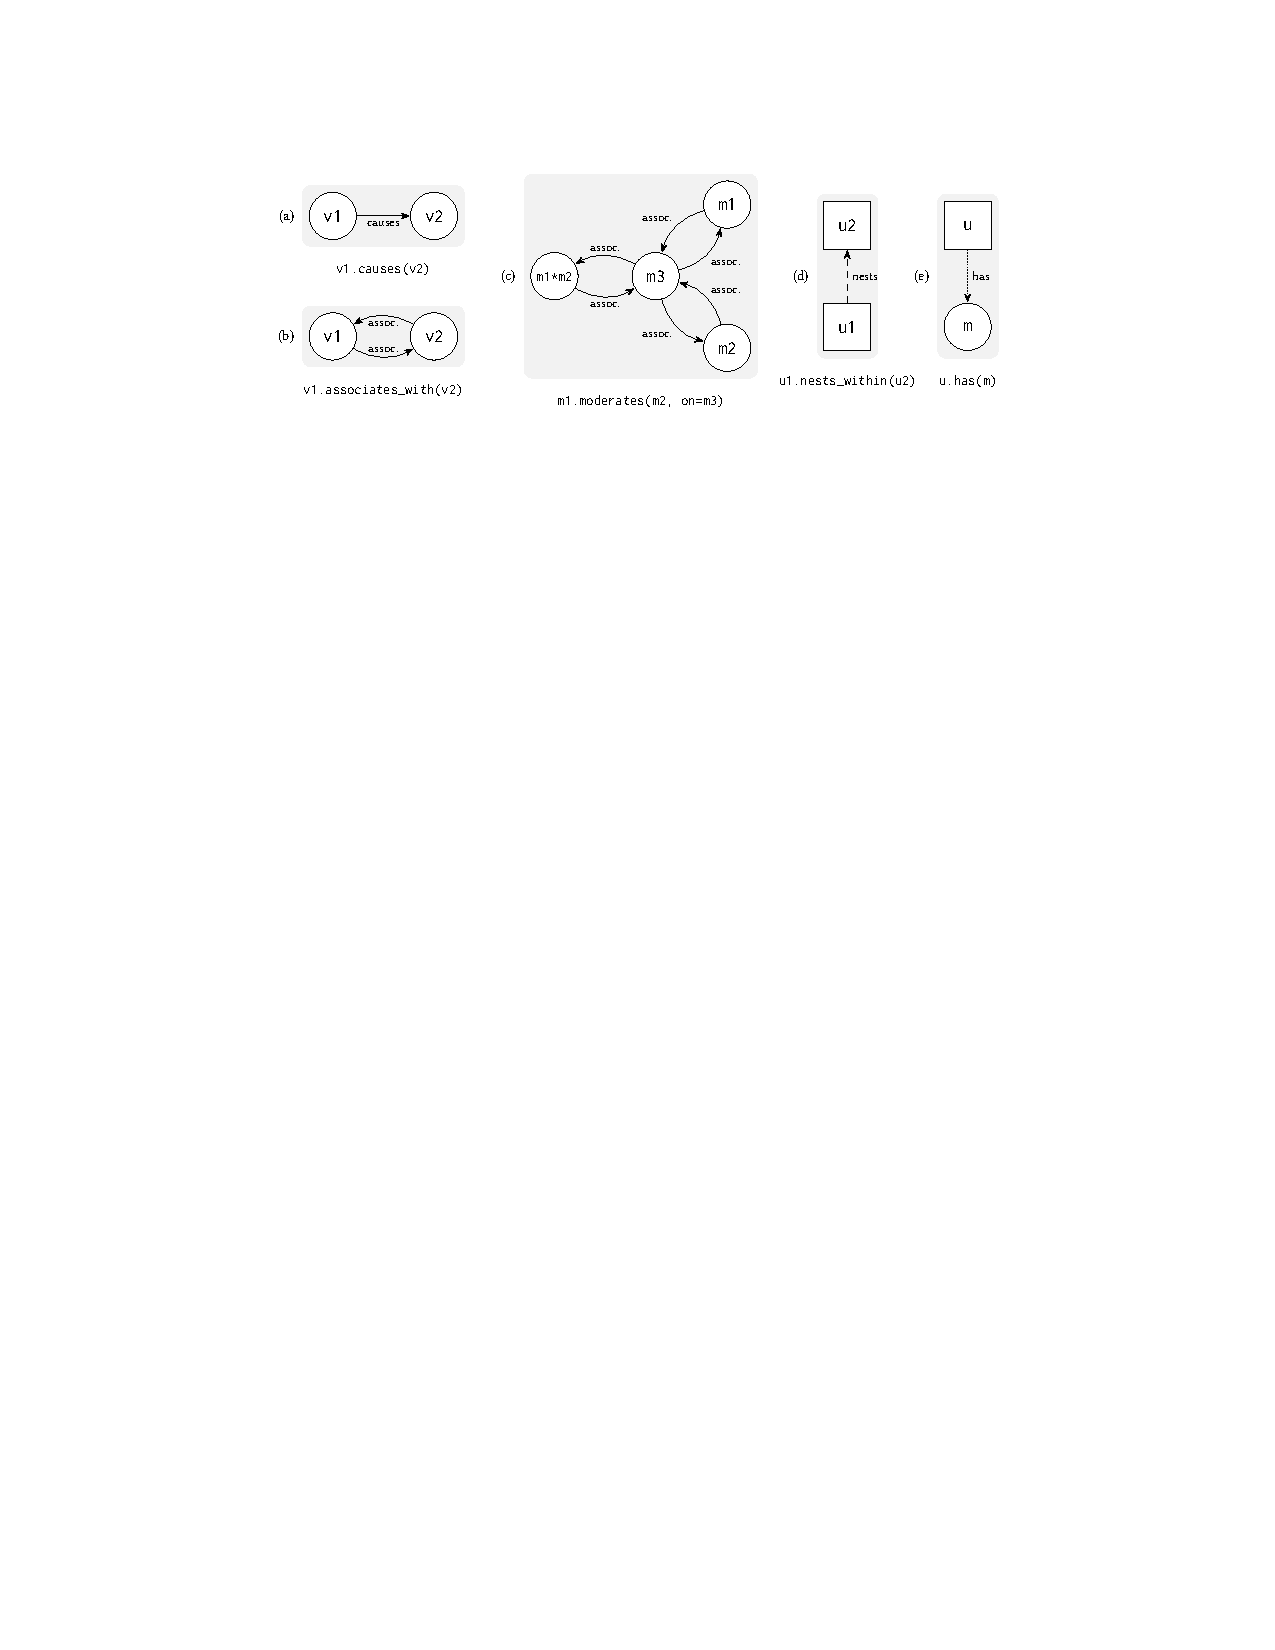
\includegraphics{tisane/figures/figure3}
%         \caption{Code snippets of conceptual and data measurement relationships written in Tisane's \SDSLlong and their representation in Tisane's graph IR. Variables are named with \texttt{u} for units, \texttt{m} for measures, and \texttt{v} for data variables that can be either units or measures. All edges depicted are those that are added due to the relationship. In the \texttt{moderates} example, we assume that \texttt{m1} and \texttt{m2} both belong to the same unit, and for simplicity, the attribution edge (labeled as ``has'') from \texttt{m1} and \texttt{m2}'s unit is not shown.}
%         \label{fig:figureSDSLToGraphIR}
%         \Description{Five directed graphs are shown. All nodes are labeled with a monospaced font. The first directed graph has two nodes, labeled “v1” and “v2”, both circles. There is a solid edge from “v1” to “v2” labeled “causes”. Below this graph is a code snippet reading “v1.causes(v2)”. The second directed graph also has two nodes, also labeled “v1” and “v2” and both circles. There are solid edges from “v1” to “v2” and from “v2” to “v1”. Both edges are labeled “assoc.” Below the graph is a code snippet: “v1.associates_with(v2)”. The third directed graph contains four nodes, which are labeled “m1*m2”, “m1”, “m2”, and “m3”. All are circles. There are six edges in the graph, all solid and labeled “assoc.” The edges are from “m1*m2” to “m3”, “m3” to “m1*m2”, “m1” to “m3”, “m3” to “m1”, “m2” to “m3”, and “m3” to “m2”. Below the graph is a code snippet: “m1.moderates(m2, on=m3)”. The fourth directed graph contains two nodes, labeled “u1” and “u2”. Both are squares. There is a dashed edge labeled “nests” from “u1” to “u2”. Below the graph is the code snippet “u1.nests_within(u2)”. The fifth, and final, directed graph contains two nodes labeled “u” and “m”. “u” is square-shaped and “m” is circle-shaped. There is a dotted edge from “u” to “m”, labeled “has”. Below the graph is the code snippet “u.has(m)”.}
%     \end{figure*}


\paragraph{Data measurement relationships.}\label{sec:data-measurement-relationships}

Study designs may have clusters of observations that need to be modeled explicitly for external validity.
For example, in a within-subjects experiment, participants provide multiple
observations for different conditions. An individual's observations may cluster
together due to a hidden latent variable. Such clustering may be imperceptible
during exploratory data visualization of a sample but can threaten external validity.
%(see~\ref{sec:validity}).
GLMMs can mitigate three common sources of clustering that
arise during data collection
~\cite{gelmanHill2006regression,kreft1998introducing,cohen1988statistical}:

\begin{itemize}
  \item \textbf{Hierarchies} arise when one observational/experimental unit
  (e.g., adult) nests within another observational/experimental unit (e.g.,
  group). This means that each instance of the nested unit belongs to one and
  only one nesting unit (many-to-one).
  % The nesting unit has multiple nested units.
  \item \textbf{Repeated measures} introduce clustering of observations from the
  same unit instance (e.g., participant).
  \item \textbf{Non-nesting composition} arises when overlapping attributes
  (e.g., stimuli, condition) describe the same observational/experimental unit
  (e.g., participant)~\cite{gelmanHill2006regression}.
\end{itemize}

The above sources of clustering pose three problems for analysts. First,
analysts must have significant statistical expertise to identify when data
observations cluster. Second, they must know how to mitigate these clusters in
their models. Third, with this knowledge, analysts must figure out how to
express these types of clustering in their analytical tools. Even if analysts
are not able to identify clustered observations, they are knowledgeable about
how data were collected.

% \enlargethispage{-12pt}

Thus, Tisane addresses the three problems by (i) eliciting data measurement
relationships from analysts to infer clusters and (ii) formulating the maximal
random effects structure, optimizing for external validity
(\ref{sec:interaction_model}). Below, we describe language features for expressing data measurement relationships.

\paragraph{Nesting relationships: Hierarchies}
\textbf{Hierarchies} arise when a unit (e.g., an \adult) is nested within another
unit (e.g., an exercise \group). Researchers may collect data with
hierarchies to study individual and group dynamics together or as a side effect of
recruitment strategies. To express such designs, Tisane provides the
\texttt{nests\_within} construct. Conceptually, nesting is strictly between
observational/experimental units, so Tisane type checks that the variables
that nest are both Units. %Tisane assumes there are multiple nested units within a nesting unit.
In the graph IR, a nesting relationship is encoded as an edge between two unit
nodes (\ref{fig:figureSDSLToGraphIR}(d)). There is one edge from the nested
unit (e.g., \adult) to the nesting unit (e.g., \group)~\footnote{The GitHub repo contains a gallery of examples that include nesting relationships.}.

\paragraph{Frequency of measures: Repeated measures, Non-nesting composition}
\def\numberofinstances{\texttt{number\_of\_instances}\xspace}
When a measure is declared through a unit, Tisane adds an
attribution edge (``has') from a unit node to a measure node (\ref{fig:figureSDSLToGraphIR}(e)).
A unit's measure can be taken one or more times in a study. The frequency of
measurement is useful for detecting repeated measures and non-nesting
composition. In \textbf{repeated measures} study designs, each unit provides
multiple values of a measure, which are distinguished by another variable,
usually time. \textbf{Non-nesting}~\cite{gelmanHill2006regression} composition
arises when measures describing the same unit overlap. For example, HCI researchers studying input devices might
design them to utilize different senses (e.g., touch, sight, sound).
Participants in the study may be exposed to multiple different devices, which
act as experimental conditions of senses. The conditions are intrinsically tied to the
devices, and participants can be described as having both conditions and
devices, which overlap with one another. Such study designs
introduce dependencies between observations~\cite{clark1973language} and hence
violate the assumption of independence that GLMs make.

\def\inputdevice{\texttt{device}\xspace} When analysts declare Measures, they
specify the frequency of the observation through the
\texttt{number\_of\_instances} parameter. This parameter accepts an integer,
variable, a Tisane \texttt{Exactly} operator, or a Tisane \texttt{AtMost}
operator. By default, the parameter is set to one. The \texttt{Exactly} operator
represents the exact number of times a unit has a measure. The \texttt{AtMost}
operator represents the maximum number of times a unit has a measure. Both
operators are useful for specifying that a measure's frequency depends on
another variable, which is expressible through the \texttt{per} function. For
example, participants may use two \inputdevice{}s \textit{per}
\texttt{condition} assigned: \texttt{device = subject.nominal(\upquote{Input
device}, number\_of\_instances=ts.Exactly(2).per(condition))}. \polish{Overruns column?} The \texttt{per}
function uses the Tisane variable's cardinality by default but can instead use a
data variable's \numberofinstances by specifying \texttt{use\_cardinality=False}
as a parameter to \texttt{per}. Moreover, specifying a measure's
\texttt{number\_of\_instances} to be an integer is syntactic sugar for using the
\texttt{Exactly} operator. Specifying a variable is syntactic sugar for
expressing \texttt{ts.Exactly(1).per(variable)}.

To determine the presence of repeated measures or non-nesting composition,
Tisane computes the \numberofinstances of measures and their relationship to
other measures. Measures that are declared with \numberofinstances equal to one
are considered to vary between-unit. Measures that are declared with
\numberofinstances greater than one or a variable with cardinality greater than
one are considered to vary within-unit as repeated measures. If there are
instances of a measure per another measure sharing the same unit, the measures
are non-nesting.

%     \begin{figure}[h]
% \centering
% 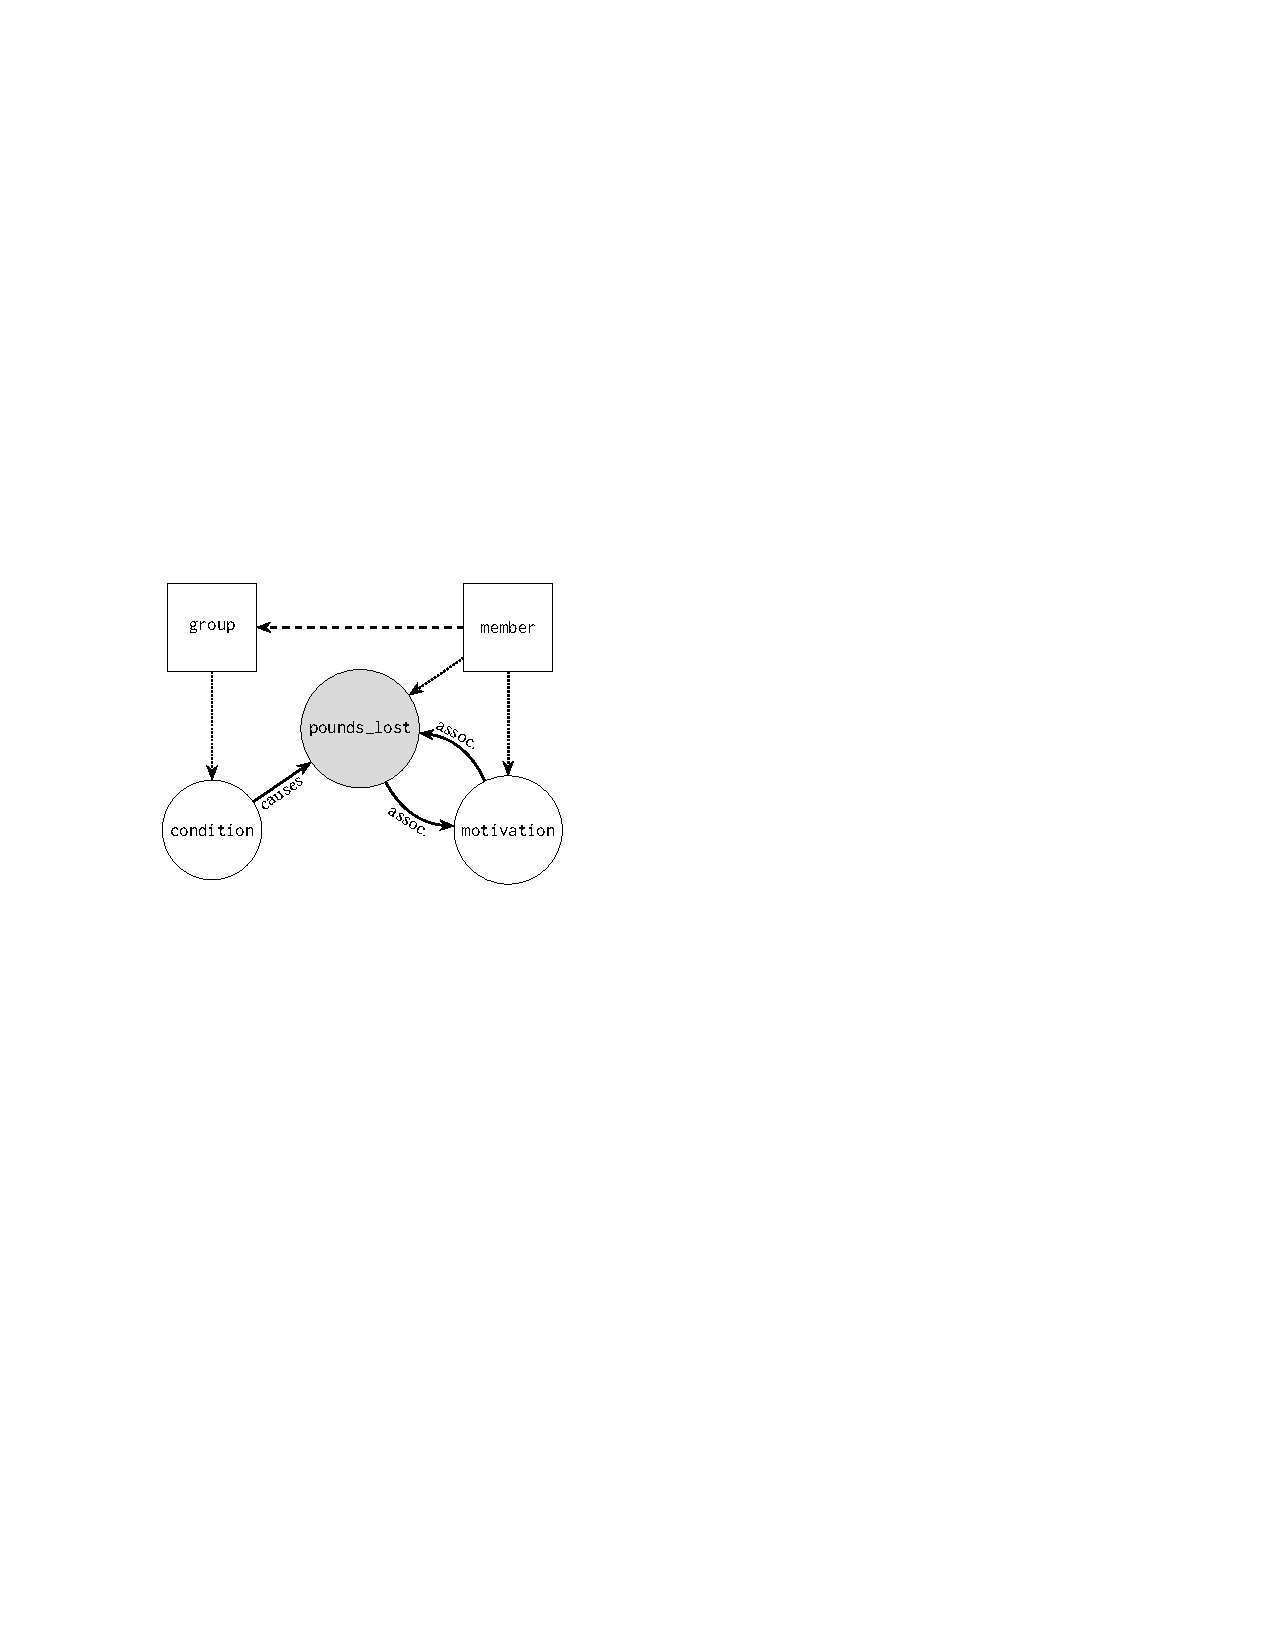
\includegraphics{tisane/figures/figure4}
%         \caption{The graph representation of the variables and relationships from the usage scenario. \texttt{causes} edges are labeled with ``causes''. \texttt{associates\_with} edges are labeled with ``assoc.'' Dashed edges indicate \texttt{nests\_within} relationships, and dotted edges indicate \texttt{has} relationships.}
%         \label{fig:figureGraphIRExample}
%         \Description{A directed graph of five nodes is depicted. The nodes are labeled “group”, “condition”, “pounds_lost”, “motivation”, and “member”, all in monospace font. The “group” node is square-shaped (indicating the node represents a Unit), and has a dotted edge pointing to the circle-shaped (indicating it's a Measure) “condition” node. The “condition” node has a solid edge labeled “causes” pointing to the circle-shaped, gray “pounds_lost” node. The gray color indicates that “pounds_lost” was the dependent variable. The “pounds_lost” node has one outgoing solid edge labeled “assoc.” (for associative relationships), to the circle-shaped node “motivation.” The “motivation” node has an outgoing, solid “assoc.” edges to the “pounds_lost” node. The final node, “member,” is square-shaped and has a dashed outgoing edge to the “group” node and dotted outgoing edges to the “pounds_lost” and “motivation” nodes. The dashed edge means “member” nests in “group” and the dotted edges mean that “pounds_lost” and “motivation” are measures of the “member” unit.}
%     \end{figure}

\subsection{Statistical model inference: Interactively querying the graph IR}
\label{sec:interaction_model} After specifying variable relationships, analysts
can query Tisane for a statistical model. Queries are constructed by specifying
a study design with a dependent variable (the value to be predicted) and a set
of independent variables (predictors). Tisane processes the query and generates
a statistical model in four phases: (1) preliminary conceptual checks that
validate the study design, (2) inference of possible effects structures and
family and link functions, (3) input elicitation to disambiguate possible
models, and (4) generation of a final executable script, and a record of decisions during disambiguation. Given that the interactive process begins with
an input program using Tisane and outputs a script for fitting a GLM or GLMM, we
call this process \textit{interactive compilation}.

\subsubsection{Preliminary checks} \label{sec:prelim-checks}
At the beginning of processing a query, Tisane checks that every input study
design is well-formed. This involves two conceptual correctness checks. First,
every independent variable (IV) in the study design must either cause or be
associated with the dependent variable (DV) directly or transitively. Second, the
DV must not cause any of the
IVs, since it would be conceptually invalid to explain a
cause from any of its effects. If any of the above checks fail, Tisane
issues a warning and halts execution. By using these two checks, the Tisane
compiler avoids technically correct statistical models that have little to no
conceptual grounding (\dcConceptualKnowledge). If the checks pass, Tisane proceeds to the next phase.
% Tisane ensures that any statistical model it infers is both conceptually and
%technically valid relative to the analyst's specified relationships.

\subsubsection{Candidate statistical model generation}
A GLM/GLMM is comprised of a model effects structure, family function, and link
function. The model effects structure may consist of main, interaction, and
random effects. Tisane utilizes variables' conceptual relationships to infer candidate
main and interaction effects and data measurement relationships to infer
random effects. Tisane infers family and link functions based on the data type
of the DV in the query. The candidate statistical models that Tisane
generates, based on the graph and query, seed an interactive disambiguation
process.

The purpose of identifying candidate main effects beyond the ones analysts may
have specified is to provoke consideration of erroneously omitted variables that
are conceptually relevant and pre-empt potential confounding and
multicollinearity issues that may arise.

\paragraph{Deriving Candidate Main Effects}
In a query to infer a statistical model, analysts specify a single dependent
variable and a set of one or more IVs. After passing the checks described in~\ref{sec:prelim-checks}, %As described above, the input IVs are
%checked to make sure that they have conceptually causal or associative %relationships. %Given that they do,
the query's independent variables are considered candidates. In addition, Tisane
derives three additional sets of candidate main effects intended to control for
confounding variables in the output statistical model\footnote{Tisane currently
treats each input IV as a separate ``exposure'' variable for which to identify
confounders. Tisane then combines all confounders into one statistical model.}.
The first two sets below are from the ``modified disjunctive cause
criterion''~\cite{vanderweele2019modifiedDisjunctiveCriterion}:

\begin{itemize}    
    \item \textbf{Causal parents.} For each IV in the query, Tisane finds its
    causal parents (see~\ref{fig:figureCandidateMainEffects}(a)).
    % , as recommended
    % by~\cite{vanderweele2019modifiedDisjunctiveCriterion}.
    \item \textbf{Possible causal omissions.} Tisane looks to see if any other
    variables not included as IVs cause the DV 
    % , as recommended
    % in~\cite{vanderweele2019modifiedDisjunctiveCriterion} 
    (see
    in~\ref{fig:figureCandidateMainEffects}(b)). They are relevant to the DV
    but may have been erroneously omitted.
    \item \textbf{Possible confounding associations.} For each IV, Tisane looks
    for variables that are associated with both the IV and the DV (see
    in~\ref{fig:figureCandidateMainEffects}(c)). Because associations
    between variables can have multiple underlying causal structures, Tisane
    recommends variables with associative relationships with caution. Tisane
    issues a warning describing when not to include such a variable in the GUI.
\end{itemize}

\figureCandidateMainEffects

%     \begin{figure*}%[h]
% \centering
% 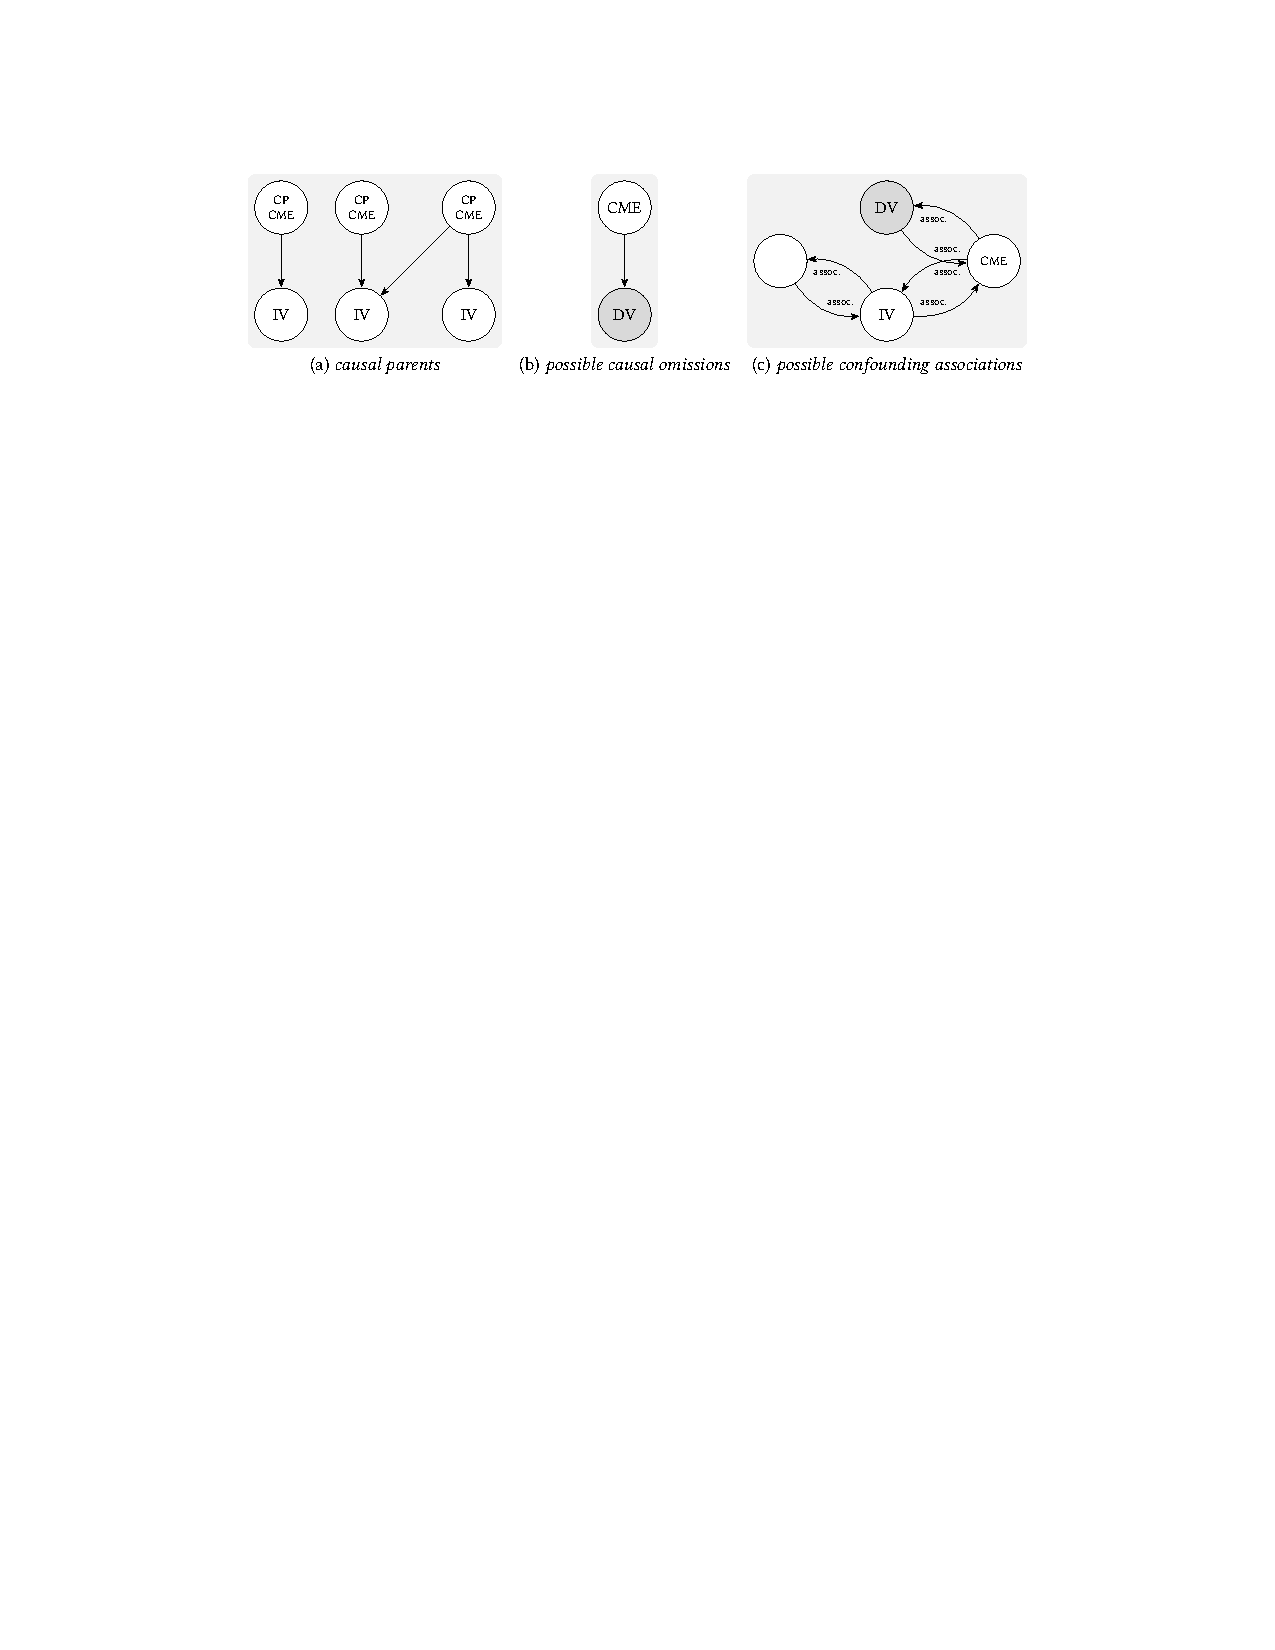
\includegraphics{tisane/figures/figure5}
%         \caption{Graphs demonstrating causal parents, possible causal omissions, and possible confounding associations. In graphs (a) and (b) (left and middle), all edges are causal. Independent variables are marked ``IV'', discovered candidate main effects ``CME'', dependent variables ``DV'', and causal parents ``CP''.}
%         \label{fig:figureCandidateMainEffects}
%     \end{figure*}

Using the above rules, Tisane suggests a set of variables that are likely
confounders of the variables of interest expressed in the query. There may be
additional confounders due to unmeasured or unexpressed variables that are either
not known or excluded from the graph. Tisane never automatically includes the
candidate main effects in the output statistical model. Analysts must always
specify a variable as an IV in the query or accept a suggestion (\dcGuidance).

If a graph only contains associates edges then the candidate main effects Tisane
suggests are those that are directly associated with both the DV and an IV. If a
graph has only causal edges, Tisane would suggest variables that directly cause
the DV but were omitted from the query and the causal parents of IVs in case the
parents exert causal influence on the DV through the IV or another variable that is not
specified.

The total set of main effects, including variables the analyst has specified as
IVs in their query and candidate main effects, are used to derive candidate interaction
effects and random effects, which we discuss next.

% However, relying on formal causal analysis to guide modeling is insufficient,
% and additional methods for ensuring conceptual validity are necessary.
\paragraph{Deriving Candidate Interaction Effects}
An interaction between variables means that the effect of one variable (the \textit{moderated} variable) on a \textit{target} variable is moderated by another (non-empty) set of variables (the \textit{moderating} variables). Tisane's
\SDSL already provides a primitive, \texttt{moderates}, to
express interactions. As such, Tisane's goal in suggesting candidate interaction
effects is to help analysts avoid omissions of conceptual relationships
that are pertinent to an analyst's research questions or hypotheses (\dcConceptualKnowledge).
Candidate interaction effects are the interaction nodes whose (i) moderated and moderating variables include two or more candidate main effects and (ii)
    target variable is the query's DV.

\paragraph{Deriving Candidate Random Effects} \label{sec:deriveRandomEffects}
Random effects occur when there are clusters in the data, which occur when
we have repeated measures,
nested hierarchies, or non-nesting composition (as defined in subsection~\ref{sec:data-measurement-relationships}). Tisane implements Barr et al.'s recommendations
for specifying the maximal random effects structure of linear mixed effects
models for increasing the generalizability of statistical
results~\cite{barr2013random, barr2013randomUpdated}.

To derive random effects, Tisane focuses on the data measurement edges in the
graph IR. Using the graph IR, Tisane identifies unit nodes, looks for any nesting
edges among them, and determines within- or between-subjects
measures based on the frequency of observations for units. % by using metadata stored in the attribution edges about the number of
%observations each unit has of any particular measure.
From these, Tisane
generates random intercepts of units for the unit's measures that are between-subjects as well as the unit's measures that are within-subjects where each instance of the unit
has only one observation per value of another variable. Tisane generates random slopes of a unit and its measure for all measures
that are within-subjects where each instance of the unit has multiple
observations per value of another variable. For interaction effects, random
slopes are included for the largest subset of within-subjects variables (see~\cite{barr2013randomUpdated}). %,
%according to Barr's updated recommendations~\cite{barr2013randomUpdated}.
Tisane handles correlation of random slopes and intercepts during disambiguation (subsection~\ref{sec:disambiguation}).
%When there are both random slopes and random intercepts for the same unit, Tisane asks analysts if they are correlated during disambiguation. By default, Tisane assumes correlation.
% due to computational limitations or insufficient data,
Maximal random effects may lead to model convergence issues that analysts
address by later removing or adding independent variables and random effects. Nevertheless, starting with
a maximal, valid model is important for ensuring that future revisions are also valid (\dcValidity).

\paragraph{Deriving Candidate Family and Link Functions} \label{sec:family_link_functions}
The DV's data type determines the set of candidate family and
link functions. For example, numeric % or continuous data
variables cannot have
binomial or multinomial distributions. Similarly, nominal variables are not
allowed to have Gaussian distributions. Furthermore, each family has a set of
possible link functions. For example, a Gaussian family distribution may have an
Identity, Log, or Square Root link function. The statistics literature documents
    possible combinations of family and link functions for specific data
types~\cite{nelder1972generalized}.
%  that software tools such as
% statsmodels~\cite{statsmodelsRef} and lme4~\cite{bates2014fittingLme4}
% implement.

Tisane includes common family distributions as candidate families and their
applicable link functions. In its current implementation, Tisane relies on
\statsmodels~\cite{statsmodelsPaper} for GLMs and
\texttt{pymer4}~\cite{jolly2018pymer4} for GLMMs. As such, Tisane is limited to
the family and link function pairings implemented in these
libraries.~\autoref{tab:tableFamilyLinkFunctions} lists the family and link
functions these libraries currently supports. As \statsmodels' and \pymer's
support for GLMs grows in the future, Tisane can be extended.
% Tisane can be
% extended to take advantage of new family and link implementations in these
% libraries.

\tableFamilyLinkFunctions

\subsubsection{Eliciting Analyst Input for \Disambiguation}\label{sec:disambiguation}
\groupExerciseDisambiguation
% Upon generating a set of candidate main, interaction, and random effects, Tisane
% asks analysts questions before outputting a statistical model.
The disambiguation process provides an opportunity for analysts to explore the
space of generated models based on their original query. Given our design
considerations to prioritize conceptual knowledge (\dcConceptualKnowledge) and
give analysts guidance (\dcGuidance), we designed a GUI to scaffold analysts' reasoning and elicit their input.
For versatility, we implemented Tisane's GUI using Plotly
Dash~\cite{plotlyDash}. Analysts can either execute their Tisane programs and use the
GUI inside a Jupyter notebook (no additional widgets needed) or run
their Tisane programs in an IDE or terminal, in which case Tisane will open the
GUI in a web browser. 
% Figure~\ref{fig:groupExerciseDisambiguation}
% gives an overview of the GUI.

% Tisane grounds explanations and disambiguation questions in the
% variable relationships analysts declared in their input Tisane program,
% for explaining why specific generated main and interaction effects may be
% desirable, how Tisane automatically inferred the random effects structure, and
% show data distributions to help analysts select family and link functions (Figure~\ref{fig:groupExerciseDisambiguation}).
Candidate statistical models are organized according to (i) independent
variables  (main effects and interaction effects), (ii) data clustering (random
effects), and (iii) data distribution (family and link functions). In the main
effects tab, Tisane asks analysts if they would like to include additional or
substitute main effects that Tisane infers to be conceptually relevant. In the
interaction effects tab, Tisane suggests moderating relationships to include but
does not automatically include them because analysts may not have specific
hypotheses involving interactions (\dcGuidance). If analysts do not specify any
moderating relationships, Tisane does not suggest any interaction effects,
preventing analysts from including arbitrary interactions that may be
conceptually unfounded (\dcConceptualKnowledge, \dcValidity).

In the data clustering tab, Tisane shows analysts which random effects it
automatically includes based on the selected main and interaction effects. Unlike
main and interaction effects, Tisane automatically includes random effects
in order to maximize model generalizability (\dcValidity). If there is a random
slope and random intercept pertaining to the same unit, Tisane asks analysts if
they should be correlated or uncorrelated. We provide this option because
analysts may have relevant domain expertise to make this decision (\dcGuidance).
By default, Tisane correlates the random slope and random intercept.

The final tab, data distribution, helps analysts examine their data and select
an initial family and link function to try. Appropriate selection of family and
link functions depends on the data type of the dependent variable and the
distribution of model residuals. Therefore, the selection can only be assessed
after choosing a family and link function in the first place.

For an initial statistical model to consider, Tisane narrows the set of family
functions considered based on the declared data type of variables
(see~\ref{sec:family_link_functions}) and lightweight viability checks, such
as ensuring that a Poisson distribution is only applicable for variables that
have nonnegative integer values. Tisane asks questions designed to uncover
more semantically meaningful data types (e.g., counts) than are provided at
variable declaration. Analysts without data can answer these questions as they
are planning their studies (\dcStatisticalPlanning). For the selected family
candidate, Tisane automatically selects the default link function based on the
defaults for \statsmodels~\cite{statsmodelsRef} and
\texttt{pymer4}~\cite{jolly2018pymer4}. Analysts can then choose a different
link function, as long as it is supported.
% \footnote{See supplemental material for
% a complete listing of Tisane's supported family and link function pairings.}.}
% We chose to ask these questions during
% disambiguation rather than provide additional data types to Tisane's \SDSL to
% simplify the variable declaration process. \ej{Not sure I believe this.}}

\subsubsection{Output}
There are two outputs of the interactive compilation: (ii) an executable modeling script and (ii) a log of GUI
choices. To increase transparency of the
authoring process, Tisane provides a log of user selections in the GUI as
documentation, which the analyst can include in pre-registrations, for example
(\dcStatisticalPlanning). In the output script, Tisane includes code to fit the
model and plot residuals against fitted values in order to assess the
appropriateness of family and link functions, as is typical when examining
family and link functions. The output script also includes a comment explaining
what to look for in the plots and an online resource for further reading. Should
analysts revise their choice of family and link functions, they can re-generate
a script through the Tisane GUI.

% \section{Initial Evaluation: Case studies with real-world researchers}
\section{Initial evaluation: Case studies with researchers}\label{sec:tisane_case_studies}
Given Tisane's novel focus on deriving and
guiding analysts toward valid statistical models, we assessed how Tisane affects
data analysis practices in three case studies with researchers. The following research questions guided
the evaluation:
\begin{itemize}
    \item \rqWorkflow How does Tisane's programming and interaction model
    affect how analysts author models? Specifically, what does Tisane make
    noticeably easier or more difficult when conducting an analysis?
    %Where do researchers find themselves spending more time or attention
    %compared to without Tisane? % What are you doing? not doing?
    \item \rqCognitive Where do researchers report spending more
    time or attention when using Tisane? How does this compare to their
    fixation during analyses typically?
    \item \rqFuture When do researchers imagine using Tisane
    in future projects, if at all? What additional support do researchers want
    from Tisane? 
\end{itemize}

We recruited researchers through internal message boards and individual
contacts. We intentionally recruited researchers at different stages of the
research process---study planning, data analysis for publication, and ongoing
model building and maintenance. We believed this could help us more holistically
evaluate Tisane's impact on data analysis. We met with researchers over Zoom
[R1, R3] and in person [R2] to discuss their use cases, observe them use
Tisane for the first time, and ask for open-ended feedback. We pointed researchers to the Tisane tutorial for
installation instructions and examples but otherwise encouraged the researchers
to work independently. We answered any questions researchers had while using Tisane.
Each study session lasted approximately 2 hours. At the end, two of the three
researchers [R1, R3] said they planned to use Tisane again over the next two months.

\subsection{Case Study 1: Planning a New Study}
R1, a clinical psychology PhD student, had recently submitted a paper and was
planning a follow-up.
% to ask based on knowing how to author models she
% understood conceptually but had low confidence specifying correctly on her
% own.
R1 reported that she had never taken a formal class on modeling techniques but
taught herself for her last paper. Her general workflow involved consulting with
and mirroring what others in her research group did even if she did not
completely understand why. R1 did not program often but said she had ``enough
coding experience to understand this kind of...[sample program].'' Although
familiar with Python, R1 preferred M+~\cite{mplus} and SPSS~\cite{spss}. She was
interested in using Tisane to brainstorm new studies and research questions.

\textit{Using Tisane.} After installation, R1 read through one of the
computational notebook examples available in the Tisane GitHub repository.
While reading, R1 asked clarifying questions about the variable types and
syntax. R1 explained that the \texttt{Design} class felt novel because she had
never seen the concept of a study design in data analysis code before. When the
first two authors explained that it was supposed to be the equivalent of the
statement of a study design in a paper, R1 remarked that usually, she ``[kept]
that in [her] head, which [she] probably shouldn't'' (\rqCognitive). Without
a concrete data set, R1 preferred to walk through more examples %and discuss how
%their Tisane program would differ
rather than author a script of her own.

While reading an example, R1 drew a parallel between the tabs in SPSS dialogs for specifying models and
the tabs in the Tisane GUI, noting that SPSS had a tab for control variables.
R1 also wanted the ability to distinguish between ``control
variables'' and other independent variables in the Tisane GUI. R1 explained that this
would map more closely to how psychologists think about analyses.
Future work could incorporate additional language constructs, such as
a new data type for controls, for different groups of users (\rqFuture).
% This feedback
% suggests that future work could examine additional language constructs, such as
% a new data type for controls, would be helpful for different groups of users (\rqFuture).

\begin{comment}
R1 explained how in the past, she had run a series of tests only to learn later
that she should have been using GLMs. Even when she constructed the GLMs, %linear models,
she expressed uncertainty about her choice of family function: ``I don't know
[what] I was exactly picking...like Poisson regression or whatever.''
% ...I honestly, admittedly did not really look into which I should have been picking...but I just had one of [a colleague's] previous students [say],
R1 explained that she was given little guidance on choosing a model; another
student just told her, ```This is what I did. So you should just do that.''' In
contrast, R1 really liked having the normality checks and data histograms
available in the Tisane GUI to be more aware of the data (\rqCognitive).
\end{comment}

At the end of the study session, R1 remarked how Tisane ``fills in a lot of
the...gaps'' in data analysis (\rqWorkflow, \rqCognitive). The first gap R1
discussed was the \emph{programming gap} between scientists and statistical
tools. R1 believed that, for scientists who were not comfortable with
programming, ``they should probably be running less complex models, or first
learn how to code'' even if the complex models would be most appropriate. The
second gap R1 discussed was the \emph{statistical knowledge gap} in tools. R1 explained that
in her experience, R provides support for more complex models but little
guidance for what those models or statistical tests should be, requiring ``top
down assumption[s].'' Thus, to R1, Tisane bridged the gap between tools like
SPSS and R by requiring minimal programming and providing modeling support. Put
another way, Tisane bridged the gulf of execution~\cite{norman2013doet} for R1
that previous tools had not.
% conflation of programmign and analysis skills, making it easier for people to
% author models who may not be programmers yet need to for their work/research

% R1
% mentioned that in clinical psychology, it is often not possible to find causal
% relationships, and was more interested in finding novel correlations in the data.
% R1 was at the planning stage of data analysis, and was


\subsection{Case Study 2: Analyzing Data for a Paper Submission}
% \textit{Analysis task.}
R2, a computer science PhD student, had conducted a within-subjects study where
47 participants used four versions of an app for one week each (four
weeks total). The motivating research question was how the different app designs
led to %levels of
psychological dissociation. % during usage.
% R2 had logged
% self-report survey responses, click behavior, and time spent in %on specific elements of
% the app.
Although R2 had expected to collect multiple survey responses for each
participant each day, they only had
aggregate daily self-report measures due to an error in the database management system.
% As a result, R2 was
% unsure about which models to use for the aggregated ordinal
% data. % and which models to use.
%Using lecture notes from a past statistics course,
In the past, R2 reported having extensively explored their data and
consulting others, but for this paper, they had not explored their data prior to
fitting models because they felt more confident in their modeling skills. For
analyses, R2 preferred R but had general Python programming experience. Prior
to using Tisane, R2 had authored linear mixed effects models in R for their
study. They were interested in using Tisane to check their analyses prior to
submitting their paper to CHI.


\def\numberofinstances{\texttt{number\_of\_instances}\xspace}


\textit{Using Tisane.} %R2
%wrote two scripts using Tisane over the course of two hours.
R2 wrote their scripts by adapting an
example from the Tisane GitHub repository.
% While authoring
% their scripts, R2 read the API documentation and examples closely and found
% \texttt{SetUp} variables novel but understandable.
% After a brief explanation, R2 specified date of study to be a \texttt{SetUp} variable.
As R2 considered which conceptual relationships to add, they reasoned aloud about
if they should state causal or associative relationships between various measures and dissociation (\rqCognitive). % R2 found stating conceptual relationships difficult, stating:
%On one hand, ``[a participant] taking [one of the recorded
%actions] [does not spark] dissociation for them,'' but on the other hand,
%``dissociation might be causing them to...take that action.'' 
After some
deliberation, they said, ``I don't feel comfortable [making a causal
statement],'' and instead specified \texttt{associates\_with} relationships.
R1's hesitation to assert causal relationships confirms prior findings that
specifying formal causal graphs is difficult for domain
researchers~\cite{suzuki2020causal,suzuki2018mechanisms,velentgas2013developing} and our design choice
to allow for association edges.
% ``Because...for instance, if people use like a dialog exit to leave an app, that doesn't...cause them to dissociation...them taking that action is not sparking dissociation for them, but...dissociation might be causing them to...take that action....I don't feel comfortable [making a causal statement]. We can just say it's associated.''
In addition, R2 was initially unsure about how to specify the
\numberofinstances for their measures since their original study design
was unbalanced. %Participants could have varying numbers of measures logged per day.
After asking for clarification about \numberofinstances,
R2 declared all the measures with the parameter
\numberofinstances set equal to \texttt{date}.
% Given that they had decided to aggregate measures for each day for each
% participant,
% R2 reasoned that they could specify the measures to repeat once for
% each day in the study by declaring all the measures with the parameter
% \numberofinstances set equal to \texttt{date}.

Next, R2 ran their script %from the terminal
and used the Tisane GUI in a browser window. Based on Tisane's recommended
family and link functions, R2 realized the models they had previously authored
in R using a Gaussian family were inappropriate. Due to a bug that we have since
fixed, Tisane suggested a Poisson family that R2 used to generate a script, but
this was an invalid choice given that not all dependent variable values were
nonnegative integers. R2 explored other family distributions and generated a new
script using an Inverse Gaussian family. When executed, the second output script
issued an error due to the model inference algorithm failing to converge.
R2 made a note to look into this model further on their own.

\begin{comment}
Based on Tisane's reported normality test
results, they realized they could not assume their data were normally
distributed and that using a linear mixed effects model was inappropriate.
Although exploratory data analysis (EDA) would have led to the same insight, R2
said they had skipped EDA. %visualizing
%their data
%before fitting models.
As such, Tisane could help researchers %like R2
familiarize themselves with data and return to EDA (\rqWorkflow, \rqCognitive).
Upon seeing the histogram of their data overlaid with simulated data, R2
initially picked the Poisson family and executed Tisane's output script, but R2
received a model fitting error because not all dependent variable values were
nonnegative integers. We have since implemented an additional check to ensure
that Poisson is a choice only when all dependent variable values are nonnegative
integers.
% (since they were averages). Realizing that a Poisson model was inappropriate,
R2 explored the other family distributions and generated a new script using an
Inverse Gaussian family. The new output script issued an error due to the model
inference algorithm failing to converge. R2 made a note
%in their R Markdown file
to look into Inverse Gaussian distributions. %The analyst experienced similar issues for their second dataset and script.
%In the past, R2 had tried every single model, even picking one they
%had never heard of before
\end{comment}

Once finished using Tisane, R2 commented that their analysis with Tisane was more streamlined (\rqWorkflow) in contrast
to their very first paper where they had tried ``every
single kind of model that [they] could'' until finding ``the one that fits best,''
%This is the one I'm gonna use.' And I had to explain why I was using it because it was like
even if it was ``one that no one would have heard of.''
R2 also stated they would be interested in using Tisane earlier
in their analysis process in the future (\rqFuture).
%In addition, they reported being more focused on ``<fill in.>`` %(\textit{cognitive impact}).
Based on their experience with Tisane, R2 questioned their previously authored linear mixed effects model, and said it was ``unnerving'' to
discover an issue so close to a deadline. At the same time, they expressed, ``if it's incorrect, I should know
before I submit.'' A day after the study, R2 contacted the authors to inform them that they had decided to
update their analyses from linear mixed effects models to generalized linear
mixed effects models. They reported using the Inverse
Gaussian family after visualizing and checking the distribution of residuals
with help from the output Tisane script. The Inverse Gaussian family was
appropriate because their dependent variable's values were all nonnegative and
displayed a slight positive skew.
% R2 was still in the process of re-analyzing
% their second dataset.
R2's experience with Tisane suggests that Tisane can help
researchers catch errors and lead them to re-examine their data, assumptions,
and conclusions.

\subsection{Case Study 3: Developing Models to Inform Future Models}
Employed on a research team, R3 analyzes health data at the county, state,
and national levels to estimate health expenditure and inform public policy. R3
develops initial models that are used to validate and generate estimates for
larger, more comprehensive models.
% using a minimal set of covariates that will not be included in the final models was a primary concern.
Due to the
scale of data and established collaborative workflows, R3 typically works in a
terminal or RStudio through a computing cluster and had very little experience
with Python. Despite working on statistical models every day, R3 described himself as
``not...a great modeler.''
% He also appeared to be the most experienced R user among the
% researchers in our pilot and case studies.
R3 was interested in using Tisane to
determine what variables to include as random effects in a model.
% He had a limited number of variables to include in his model.

\def\statename{\texttt{state\_name}\xspace}
\def\yearid{\texttt{year\_id}\xspace}
\def\cardinality{\texttt{cardinality}\xspace}

\textit{Using Tisane.} R3 used Tisane in a local Jupyter notebook as well as on
his team's cluster. R3 used the Tisane API overview reference material on GitHub
to start writing his program, which involved copying and pasting the functions
with their type signatures and then modifying them to match his dataset and
incrementally running the program. The most common mistake R3 made while
authoring his Tisane program was to refer to variables using the string names in
the dataset (e.g., \texttt{"year"}) instead of the variable's alias (e.g.,
\yearid), an idiom common in R but not in Python.

While authoring his Tisane program, R3 found the \numberofinstances parameter
redundant, especially because his data is always ``square.'' Every \statename\
in his data set had 30 rows of data, corresponding to the \yearid{}s 1990-2019.
This is in contrast to R2, whose study design was unbalanced and resulted in
variable numbers of observations per participant that needed to be aggregated. Based on R3's feedback, we
added functionality to infer \numberofinstances for each unit, which analysts can inspect by
printing the variable.

% that's a statistical lack of knowledge on my hand, the fact that it's not normal. I don't know what to do with it.
While giving open-ended feedback on Tisane, R3, similar to R1, liked how Tisane helped ``fill
[the] gap in...[his] knowledge'' (\rqCognitive). Given the diversity of models
R3 works with, R3 found Tisane's focus on GLMs and GLMMs a ``little limiting'' and also
wished to make Tisane ``run without...the mouse'' in a script, as is typical in
his workflow (\rqWorkflow). Specifically, R3 described how he and his
collaborators typically want to explore a space of models and run them in
parallel. Nevertheless, R3 foresaw using Tisane in three types of modeling tasks
common in his work: (i) exploratory modeling to determine if there are any
interesting relationships between variables, (ii) authoring and comparing
multiple models for prediction, and (iii) working out the precise model
specification after identifying variables of interest (\rqFuture).

\subsubsection{System changes and Takeaways}
%However, given that (i) violations to normality assumptions may be acceptable with large enough sample sizes, 

We fixed bugs and iterated on Tisane's GUI based on feedback from
researchers. The largest change we made was to the data distributions tab. The data distributions
tab we tested with researchers visualized the dependent variables
against simulated distributions of family functions and included the results of the Shapiro-Wilk and D'Agostino and Pearson's normality tests. All three researchers
reported becoming more aware of their data due to the visualizations. However, researchers' enthusiasm for the feature made us wary that visualizing the simulated data 
could mislead less careful analysts to believe that family and link functions pertain to variable
distributions rather than the distributions of the model's residuals. 
To avoid
such errors while still helping analysts become more aware of their data, we
removed the simulated visualizations and normality tests and instead provide questions about the semantic nature of the dependent variable
% data
collected, as discussed in~\autoref{sec:disambiguation}.

Overall, Tisane streamlines the analysis process (\rqWorkflow) in part because
researchers report formalizing their conceptual knowledge into statistical
models more directly [R1, R2]. Although Tisane does not eliminate the need for
model revision, Tisane may scope the revisions analysts consider to significant
issues instead of details that may detract from the analysis goals [R2].
Additionally, researchers reported a perceived shift in their attention from
keeping track of and analyzing all possible modeling paths to their research
questions and data assumptions (\rqCognitive) while planning a new study and
analysis [R1] as well as while preparing a research manuscript [R2]. Future
adoption of Tisane may depend on the complexity of analyses (\rqFuture) [R3].
For instance, Tisane may provide a streamlined alternative to false starts due
to misspecifications for simpler analyses [R1, R2, R3]. For more complex models
and studies, Tisane may act more as a prototyping tool for statistical models,
helping researchers start at a reasonable model that they can then revise [R2,
R3]. Regardless of analysis complexity, externalizing analysts' conceptual
models in \tisane enhances documentation and communication of science,
potentially by enriching preregistered studies and analyses.

\section{Limitations and Motivation for Re-design}
While overall positive, the case studies made us aware of confusing keywords and
language constructs in \tisane. In order to improve \tisane and probe more
closely into what challenges statistical novices face when expressing their
domain knowledge, we engaged in an iterative process to re-design \tisane. We
started with a lab study using \tisane~\cite{jun2022tisane} to elicit
statistical non-experts' implicit definitions and assumptions about Tisane's
keywords and identify opportunities to refine \tisane's DSL and interactivity.

% . Observations from this study gave us ideas for
% re-designing Tisane's \SDSL. 

% Surprisingly, we found that some
% keywords and functions in \tisane were at too high a level of abstraction.
% Analysts wanted to express their conceptual relationships with greater detail
% and specificity. Analysts also wanted to express ambiguity about the a
% relationship's direction in the conceptual model. 

\section{Limitations and Motivation for Re-design}
Despite the importance of conceptual modeling to statistical analysis, it is
unknown what challenges statistical novices face when expressing their domain
knowledge. To identify what statistical non-experts want and are capable of
expressing about their conceptual models, we conducted a formative study using
\tisane~\cite{jun2022tisane}, an open-source tool designed to bridge this gap.
We found important limitations to \tisane. Surprisingly, we found that some
keywords and functions in \tisane were at too high a level of abstraction.
Analysts wanted to express their conceptual relationships with greater detail
and specificity. Analysts also wanted to express ambiguity about the a
relationship's direction in the conceptual model. 

\def\unit{\texttt{Unit}\xspace}
\def\measure{\texttt{Measure}\xspace}
\def\setup{\texttt{SetUp}\xspace}

\section{Elicitation lab study} \label{sec:exploratoryStudy}
% Motivation
% Our motivating question was, ``What implicit semantics do analysts use to construct conceptual models of how variables relate?''. 
\polish{rTisane should be (re-)introduced before this mention. Maybe note in 5.5
the goal of creating a revised Tisane version for R?: For the lab study, we
re-implemented \tisane (originally in Python) in R since (i) R is a widely used
programming language for data science and (ii) the research methods course
taught and used R.} Our aim was to increase the expressivity of \rTisane to
represent analysts' implicit domain knowledge. We used the first release of
\tisane~\cite{jun2022tisane} to probe analysts' internal processes and derive
design goals~\autoref{sec:rtisane_design_implications} for re-designing \tisane.

\subsection{Method}
%Participants
We recruited participants through a graduate-level quantitative research methods
course as a convenience sample to control recent exposure to
statistical concepts. Five computer science PhD students participated.
% All participants self-reported that they
% conducted research in programming languages or software engineering and planned
% to perform statistical analyses in future research projects. 
% \ej{Add: Approaches, mindsets of participants as they were completing the study}

% On a scale from
% one (not at all relatable) to five
% (extremely relatable), four participants indicated that the paper was relatable
% with a score of 3 or higher.
The study consisted of two parts: (i) a take-home assignment and (ii) an in-lab
session. The take-home assignment asked participants to read a recently
published CHI paper~\cite{winters2021heartbeat}\footnote{We chose the specific
paper because we believed its topic (i.e., empathetic biosignals) would be
broadly approachable and the statistical methods used (i.e., generalized linear
models) would be familiar with students enrolled in the research methods
course.} and describe the paper's research questions and hypotheses, the
authors' conceptual models, the study's design, and ways to analyze the data to
answer the research questions. The assignment was designed to ensure that
participants engaged with the paper's key ideas before coming into the lab. The
researcher reviewed each submission to prepare participant-specific questions
for a semi-structured, think-a-loud lab session. 

% used Tisane~\cite{jun2022tisane}, an open-source package for authoring
% generalized linear models with or without mixed effects, as a probe to
% understand how participants thought about and wanted to express their conceptual
% models and study designs. We 

At the start of the lab session, participants reviewed their homework submission
to remind themselves of the paper. The paper and participants' homework
responses remained available for reference throughout the study. Then,
participants completed three tasks: (i) declaring variables, (ii) expressing
conceptual models, and (iii) specifying study designs. For each task,
participants started with \tisane's language constructs to express their intent
and discussed their confusions, how they understood each presented construct,
and what they wanted to specify but could not (if applicable). The researcher repeatedly reminded
participants that the constructs presented were prototype possibilities and that
expressing their intentions was more important than using the constructs or
getting the syntax correct. Throughout, the researcher paid particular attention
to where \tisane broke down for participants and asked follow-up questions to
probe deeper into why. The researcher considered such breakdowns as openings
into semantic mismatches between the end-user and the DSL.

% Analysis 
We iteratively coded homework submissions, audio transcripts from the lab study
sessions, and lab study artifacts. We also consulted the
researcher's detailed notes from the lab sessions. 

% Based on an iteraWe conducted a content analysis of the produced code suggestions (output
% artifacts) along with a thematic analysis of the audio transcripts from each lab
% session. 

\subsection{Key Observations}
All participants demonstrated a working knowledge of the assigned paper's
motivating research questions, study design, and general study procedure. 
% Among
% the submitted conceptual models, four were a list of conceptual relationships,
% and one was a diagram. 
We made four key observations about what and how statistical non-experts wanted
to express their conceptual models: using varying degrees of specificity,
separating moderation from bivariate relationships, distinguishing between known
and hypothesized relationships, and considering alternative conceptual models.
Participants also suggested syntactic sugar options to improve the DSL's
usability. Based on these observations, we derived design goals for re-designing
\tisane (see~\autoref{sec:rTisane}).

\subsubsection{Participants express conceptual knowledge with varying details.}
Contrary to the popular belief that higher levels of abstraction are better for
end-users, we found that statistical non-experts want to
move up and down the ladder of abstraction when expressing conceptual models. 

When defining ``causes,'' P2 described ``[Causes] is...like when we teach
logic...it's like implication, right?....So I'm saying if we are observing an
emotion and...emotion observed can lead to a change in emotional perspective.''
P0, P1, and P3 contrasted a bidirectional relationship between variables,
formerly encapsulated in the \texttt{associates\_with} construct in \tisane, to
their implicit understanding of ``causes.'' For instance, P1 stated ``the most
like, utilitarian definition by if A causes B, then by changing A, I can change
B whereas \texttt{associates\_with} means that...if I can turn dial A, B might
not change.'' In addition to differentiating between causal and associative
relationships, three participants [P0, P1, P3] provided statements of
\textit{specifically how} a variable influenced another in the conceptual models
submitted as homework. For example, P0 wrote, ``Hearing a heartbeat that seems
to be aligned with visual cues makes someone feel \textit{more} strongly what
another person is feeling'' (emphasis added), specifying a positive influence of
``hearting a heartbeat'' on empathy. These observations suggest that analysts
have an intuitive understanding of causality but bluntly stating that a variable causes
another does not capture the richness or nuance of their implicit domain knowledge. 
Additional annotations about how a variable influences another are necessary.

%   in addition to vaguer statements without a clear
% positive/negative direction, such as ``Visual cues directly influence a person's
% perception of another's emotions'' [P0]. 
% The homework assignment and lab study materials may have primed participants to
% think about ``direct'' and ``indirect'' relationships and commutativity, so
% analysts' descriptions of causal relationships as ``unidirectional'' and
% associative relationships as ``bidirectional'' were not surprising [P0, P2, P3].

% how a bidirectional relationship between two variables 
% indicative of proxies measuring the same latent construct (``...for two things
% to be bi-directional and for it to be a really, really direct relationship. Like
% that just never happens in the real world without them turning out to be like
% proxies for the same exact thing.'') [P3]; and that 

\subsubsection{Participants find moderation difficult to separate from bivariate relationships.}
Participants consistently found \tisane's \texttt{moderates}
construct difficult to understand [P0, P1, P2, P3]. Participants expressed
confusion about what moderation implied about the relationship between
two variables. For example, P3 grappled with if ``moderates'' was shorthand for
expressing associative relationships between each independent variable and the
dependent variable, how moderation implies causal relationships, and if
statistical and conceptual definitions of moderation differed from each other:
``[L]et's say there's two independent variables and one dependent variable. And
each of the [independent] variables individually is not correlated with the
outcome. But if you put them together, then the correlation appears....I mean,
it's sort of a philosophical question of whether, like each of the ones
individually causes [the dependent variable] in that case. But thinking from
a...statistical perspective, I think that's a situation where you might be able
to express...language and experience level together cause lines of code but
individually they don't because no individual correlation would appear there.''
Therefore, a clear delineation between bivariate relationships and partial statistical specifications of interaction terms is necessary. 
% that (i) the semantics of moderation is unclear in
% Tisane and (ii) moderation may be easier to reason about when decomposed into
% what happens to the dependent variable when two or more independent variables
% have specific values. 
% \paragraph{Design implication: Too high level --> Remove moderates}

\subsubsection{Participants distinguish between known and suspected relationships.}
% [P0, P1, P2, P3, P4]
Participants described relationships established in prior work as
``assumptions'' or ``assertions'' to check separately from the key research
questions that tested ``suspected'' relationships. P0 described how ``maybe we
have to differentiate as to like the \textit{known} [relationships] are kind of
the things you're \textit{assuming} there's relationships between these things
whereas the \textit{suspected}...[are] the things kind of like your research
questions are saying like, `We \textit{think} there's this relationship
but...it's what we're testing for'' (emphasis added). Similarly, P4 suggested
that Tisane should warn end-users when assumptions about known relationships are
violated in a given data set: ``I would also say that it would be very handy to
be able to say, kind of \textit{assert} that language has no effect on the line
of code. And be warned if it's not the case, like if your \textit{assertion} is
not...verified automatically with the DSL, but warned...that while your
\textit{assumption} is not holding there is actually an effect, which could be
very handy on your study.'' (emphasis added). The inability to indicate
relationships that are either known or suspected in \tisane may explain why
analysts repeatedly preferred less technical verbs, such as ``influences'' [P0]
or ``leads to'' [P3]. For instance, P0 explained how she preferred
``influences'' over ``causes'' because ``I guess it's like \textit{a level of
sureness} in it in which, like, `cause' feels more confident in your answers
than `influences''' (emphasis added). Providing a way to label conceptual
relationships as assumptions or the focus of the present analysis could make
\texttt{causes} and \texttt{associates\_with}, the bivariate relationships in
\tisane, more approachable. 
% \paragraph{Design implication: Provide constructs for distinguishing betwen known and suspected relationships -->  assume/hypothesize}

% However, Tisane does not differentiate between known
% and suspected relationships, and as P4 noted, ``I don't know if everything that
% is not either specified to moderate, associate, or causes is by default,
% asserting that there is no effect,'' suggesting that the Tisane's DSL semantics
% could be more self-evident. In fact, 

\subsubsection{Participants consider alternative conceptual structures in the face of ambiguity.}
% In addition to detailing how variables influence one another, participants also
Participants grappled with what specific structures in a conceptual model meant. P1 and P3
described how a bidirectional relationship between two variables were really due
to hidden, confounding variables causing both variables. P3 described how ``in
the real world...when these bidirectional things happen, it means there's
sort of this middleman complex system. Or some like underlying process of which
[two variables are] both components...'' Another participant, P2, wondered aloud
about how even what appears like a direct relationship, may actually be a chain
of indirect or mediated relationships at a lower granularity: ``It's like Google
Maps. If you zoom out enough, that arrow becomes a direct arrow.'' These
observations suggest that while participants can deeply reflect on what could be
happening between variables conceptually, they need help exploring and
figuring out which of these structures matches their implicit understanding.
% P3's definition of associative relationships
% is consistent with an associative structure called a ``fork'' in causal DAGs.
% \paragraph{Need help exploring and picking among possible structures.}


\begin{comment}
\subsubsection{More expressivity for specifying study designs/experimental design}
**keep short**
Additional observations about expressing study design
More future work for how to express study designs

TODO: Participant as a separate construct
\end{comment}

\subsubsection{Participants expected more syntactic sugar for specifying data collection details.}
While our focus was on improving the support for conceptual modeling, we made a
few observations about challenges analysts faced when specifying data collection
details. First, analysts expected \textit{experimental conditions to be
standalone concepts}. In Tisane, experimental conditions can be specified as a
\measure of a \unit. Instead, P0 and P4 had separate conceptual categories for
conditions and measures in their mental models of study designs. P4 preferred a
separate condition data type currently unavailable in Tisane because the term
``Measure'' did not create a ``bucket'' appropriate for conditions. Second,
participants were interested in specifying trials, stimuli, and responses
elicited during each trial alongside participants: ``I want to have a trial
unit that is nested within trials, which is nested within or maybe I could just
have trial nested within Participant, but I'm not seeing a way to clearly
delineate or like to denote that'' [P1]. Future work should more closely examine
and iterate on language constructs and idioms for representing data collection
procedures. 

% In Tisane, nesting a trial within a
% participant would mean that multiple trials exist in each participant (e.g.,
% akin to how multiple children exist in a family), which even in natural
% language, does not capture what P1 wanted to convey, which was that each
% participant sees and provides responses for each trial. 
% \paragraph{Participant construct - syntactic sugar for Unit}

% P4 resorted to declaring
% condition as a \setup variable, violating the intended semantics of \setup
% variables in Tisane: ``Like it doesn't feel like the condition are measured.
% Right? I'm measuring the proxy. I'm not measuring the condition. So to me,
% that's why I'm putting the visual on the four condition as a...\setup
% variable.'' Similar to P4, when P0 saw the ``SetUp'' class, she thought it
% described conditions: ``[I]f I heard the word `setup,' I would think of more
% like conditions like, like, this person uses this IDE or this person is given
% this IDE.'' 

\subsection{Domain-Specific Language Re-design Goals} \label{sec:rtisane_design_implications} 
\polish{ It might be worth mentioning that, even if Tisane does not use some of the more nuanced annotations for model suggestion, these are valuable for externalizing analysts' conceptual models for documentation and communication (potentially including preregistration).}

Based on our lab study observations, we derived four design goals for
re-designing Tisane's DSL to more accurately capture analysts' implicit
conceptual models: 
%  about how
% participants internally represent conceptual models and study designs have three
% implications for improving the design of Tisane.

\def\optionalSpecificity{\textbf{DG1 - Optional specificity}\xspace}
\def\interactionAsPartialSpec{\textbf{DG2 - Interactions as partial specifications}\xspace}
\def\considerPossibilities{\textbf{DG3 - Consideration of possibilities}\xspace}
\def\assumeHypothesize{\textbf{DG4 - Distinction between assumed and hypothesized}\xspace}
\begin{itemize}
    \item \optionalSpecificity: Analysts should be able to provide optional
    details about how variables change in relation to each other (e.g., positive
    or negative changes in values) when describing conceptual relationships.
    \item \interactionAsPartialSpec: Analysts should annotate conceptual models with interaction terms they want to include in an output statistical model. 
    \item \considerPossibilities: When expressing ambiguous relationships, analysts should have support
    in considering and picking among multiple possible conceptual structures.
    \item \assumeHypothesize: Analysts should be able to distinguish between assumed and hypothesized relationships in their conceptual models. 
\end{itemize}

In the second release of \tisane, we addressed these goals through new language
constructs. We also supported syntactic sugar to more accurately capture
study design details. 

\polish{"We also supported syntactic sugar to more accurately capture study design details."
> Not clear to me why syntactic sugar more "accurately" captures details as opposed to more "efficiently"/"concisely".
> Also, what exactly was the sugar? If you stated this, it did not stick in my memory...}

\begin{comment}
\textbf{Deconstruct statistical constructs for clarity.}
Unsurprisingly, we found that class and function names such as ``Measure,''
``SetUp,'' and ``moderates'' confused participants. These names either suggested
informal conceptual categories or were too close to statistical jargon. As a
result, connecting a Tisane program's semantics to a mental model of study
design was challenging. Particularly insightful was participants' consternation
with the function ``moderates.'' Participants could reason about the details of
moderation relationships but did not know what the term meant or how to use it
to clearly communicate their conceptual models in detail. Using
specific,granular language constructs (e.g., pairwise relationships) and
allowing for system-gudiance to consider more complex statistical structures
(e.g., interaction effects for moderation) may help analysts more accurately
understand and use Tisane.

\textbf{Allow for conceptual ambiguity, make specificity optional.}
Despite being statistical non-experts, participants were noticeably focused on
low-level details about conceptual relationships. All participants
differentiated between known and suspected relationships and generally agreed
that known relationships should be checked for prior to assessing the suspected,
or ambiguous, ones. At the same time, when participants were confident about
some relationships, they were specific about if the relationships were
positive/negative. Welcoming ambiguity and specificity could help analysts write
and use conceptual models throughout data analysis and interpretation.

Both design implications suggest the need to re-structure Tisane's programming
and interaction models. First, Tisane's specification language needs to be more
specific and low-level. This finding is \textit{counterintuitive} because a
well-documented strategy for making programming tasks easier for non-experts has
been to raise the level of abstraction for a programming
domain~\cite{chasins2018rousillon,satyanarayan2017vega}. Yet, we have evidence
that suggests the opposite for specifying a conceptual model and study design.
Second, Tisane's specification process could be more tiered, and disambiguation
could leverage ambiguity in analysts' specification as opportunities for more
numerous intelligent suggestions and guidance. 

\todo{Mention that the focus needs to be on conceptual level, but within conceptual level, there should be opportunity to move up and down the ladder of conceptual abstraction}

%hand-offs to a reasoning engine to suggest possible analysis paths, for example. 

% the conceptual modeling and study design specification process to be more tiered

\end{comment}

\clearpage % to force the listing to start at the top of the next page
\rTisaneProgram
\section{System Design and Implementation} \label{sec:rTisane}

\rTisane consists of (i) a DSL for analysts to express their conceptual
models and (ii) interactive disambiguation steps to compile this high-level specification into a
script fitting a statistical model. 

So far, we have implemented \rTisane for GLMs. Given the breadth of findings
from the elicitation lab study, we narrowed the scope from \tisane in order to
really focus on designing and testing a set of language constructs core to
conceptual modeling. 
% Given the breadth of findings from the elicitation lab study, we decided to
% really focus on a set of language constructs core to conceptual modeling. 
% a DSL for expressing conceptual models
There are two key challenges to designing \rTisane: (i) ensuring the DSL's
constructs can express analysts' implicit conceptual models accurately and (ii) %identifying DSL primitives that 
balancing usability with rigor, allowing
analysts to express their often ``fuzzy'' conceptual assumptions without losing
precision to derive a statistical model.

% \rTisane supports a two-step process for analysts to specify conceptual models
% that are both expressive and precise. 
\def\Participant{\texttt{Participant}\xspace}
\def\Unit{\texttt{Unit}\xspace}
\def\Condition{\texttt{Condition}\xspace}
\def\Conditions{\texttt{Condition}s\xspace}

\subsection{\rTisanes Domain-Specific Language}
Like \tisane, analysts express variables, a conceptual model, and a query for a
statistical model. \rTisanes DSL prioritizes expressivity and usability 

\subsubsection{Declaring variables}
Analysts can express two types of variables: Units and Measures. Units represent
observational or experimental units from which analysts collect data (see line 5 in~\autoref{lst:rTisaneProgram}). 
A common unit is a participant in a study, so \rTisane provides syntactic sugar for
constructing a \Participant unit directly. \Participant is implemented as a wrapper for
declaring a \Unit.

Measures are attributes of Units collected in a \dataSet, so they are declared
through a Unit. Measures can be one of four
types: continuous, unordered categories (i.e., nominal), ordered categories
(i.e., ordinal), and counts (see lines 6-18 in~\autoref{lst:rTisaneProgram}). \rTisane provides syntactic sugar for declaring
\Conditions as either unordered or ordered categories. Analysts declare
unordered and ordered categories through the \texttt{categories} function.
Analysts can specify a variable is ordered by passing a list to the
\texttt{order} parameter. Otherwise, the variable is considered unordered.
Analysts can use \texttt{continuous} and \texttt{count} functions to declare
continuous and count Measures. 
% We
% chose this design to reduce the number of unique functions and better match
% semantic similarity. 


\begin{comment}
Units
syntactic sugar: `Participant'

Measures
syntactic sugar: `condition'
\end{comment}


\def\causes{\texttt{causes}\xspace}
\def\relates{\texttt{relates}\xspace}
\def\when{\texttt{when}\xspace}
\def\then{\texttt{then}\xspace}
\def\assume{\texttt{assume}\xspace}
\def\hypothesize{\texttt{hypothesize}\xspace}

\subsubsection{Expressing a conceptual model}
Once analysts have constructed variables, they can specify how these variables
relate conceptually. To do so, they construct a \texttt{ConceptualModel} and add
variable relationships to it (lines 20-31 in~\autoref{lst:rTisaneProgram}). The conceptual model %\texttt{ConceptualModel}
is represented as a graph where the variables are nodes and the relationships
are edges. 

There are two types of relationships: \causes and \relates. \causes indicates a
unidirectional influence from a cause to an effect. \causes
introduces a directed edge from the cause node to the effect node. \relates
indicates that two variables are related but exactly how is ambiguous because
the analyst is uncertain about the direction of influence. \relates introduces a
bi-directional edge  between two variables. During a disambiguation step,
\rTisane will walk analysts through possible graphical structures that a
bi-directional edge could represent (\considerPossibilities). To derive a
statistical model, \rTisane requires an analyst to assume a direction of
influence.


Towards the design goal of \optionalSpecificity, \rTisane allows analysts to
optionally specify \when and \then parameters in the \causes and \relates
functions. There are four comparisons analysts can specify in
\when and \then: \texttt{increases} (for continuous, ordered categories,
counts), \texttt{decreases} (for continuous, ordered categories, counts),
\texttt{equals} (for any measure type), and \texttt{notEquals} (for any measure
type). Supporting optional specificity is designed to (i) make the \rTisane
program an accurate document of analysts' implicit assumptions and (ii) suggest
ways to resolve conceptual ambiguity during disambiguation
(\considerPossibilities). 
% used when suggesting ways to resolve
% ambiguity in the input program during disambiguation
% (\autoref{subsec:conceptualModelDisambig}).

To add relationships to the conceptual model, analysts must assume or
hypothesize a relationship. This distinction supports how analysts distinguish
between assumed, or strongly held, and hypothesized, or more uncertain,
relationships. \rTisane requires analysts to make these explicit distinctions
(\assumeHypothesize) when adding conceptual relationships to a conceptual model.
In addition to specifying a relationship type, analysts must either \assume or
\hypothesize a relationship. 

% While analysts are thinking through and specifying \causes and \relates
% relationships, 

Analysts can also specify interactions between two or more variables by
declaring \texttt{interacts}. Interactions are annotations to conceptual models
and are added to the graph without \assume or \hypothesize. Interactions provide
additional information about existing relationships in the conceptual model
(\interactionAsPartialSpec). 
% Causes / relates (types of relationships)
% Optional specificity: when, then annotations
% Assume / Hypothesize (label relationships)
% Interactions as annotations 
% - default semantics: if labeled, interactions considered. Otherwise, not

\def\query{\texttt{query}\xspace}
\subsubsection{Querying for a statistical model}
Analysts \query \rTisane for a statistical model based on the input conceptual
model (lines 33-34 in~\autoref{lst:rTisaneProgram}). The query asks for a statistical model to accurately
estimate the average causal effect (ACE) of the independent variable on the
dependent variable. The querying process initiates the interactive compilation
process and results in an \texttt{R} script specifying and fitting a generalized
linear model. During interactive compilation, analysts engage in two loops to
disambiguate their (i) conceptual model and (ii) output statistical model. 

\subsection{Two-step Interactive Compilation}
There are two phases to interactively compiling a conceptual model to a
statistical model: (i) conceptual model disambiguation and (ii) statistical
model disambiguation. We added conceptual model disambiguation to address the
need to explore possible conceptual structures for resolving ambiguities
introduced by \relates (\considerPossibilities).

\subsubsection{Conceptual Model Disambiguation} \label{subsec:conceptualModelDisambig} 
\conceptualModelDisambiguation
The goal of conceptual model disambiguation is to make analysts' expressed
conceptual models precise enough to derive a statistical model, achieving
usability and rigor. Conceptual model disambiguation involves breaking cycles in
the conceptual model by (i) picking a direction for any \relates relationships
and/or (ii) removing edges. Cycles are necessary to break because they imply
multiple different data generating processes that could lead to different
statistical models. In this way, conceptual model disambiguation can help analysts
reflect on and clarify their implicit assumptions. 

To disambiguate conceptual models, \rTisane uses a GUI.~\autoref{fig:figureConceptualModelsDisambiguation} shows the conceptual model disambiguation interface for the input program in~\autoref{lst:rTisaneProgram}. The GUI shows a graph
representing analysts' conceptual models. If there are any \relates
relationships, \rTisane suggests ways analysts could assume a direction of
influence. Additionally, \rTisane suggests ways to break any cycles in the
conceptual model. As analysts make changes, the visible graph updates. The GUI
also explains why both these steps are necessary to derive a statistical model. 

Once analysts have disambiguated their conceptual models, \rTisane updates the
internal graph representation and derives a space of possible statistical
models. To narrow this space of possible statistical models down to one output
statistical model, \rTisane asks additional follow-up disambiguating questions. 

\begin{comment}
This problem is actually challenging because detecting all cycles in a graph is
an NP-hard problem. We adapt a version of Johnson's(?) algorithm.
\end{comment}

\subsubsection{Statistical model derivation and disambiguation}
\statisticalModelDisambiguation
To formulate possible statistical models, \rTisane considers potential
covariates to control for confounding, interactions, and family and link
functions.

To determine confounders, \rTisane uses more recent recommendations from
Cinelli, Forney, and Pearl~\cite{cinelli2020controls}\footnote{\tisane relied on
Vanderweele's recommendations for confounder
selection~\cite{vanderweele2019modifiedDisjunctiveCriterion}, but in \rTisane we
opted for more recent recommendations}. Cinelli et al.'s recommendations are
based on a meta-analysis of studies examining the impact of confounder selection
based on graphical structures on statistical modeling accuracy. By following
Cinelli et al.'s recommendations, \rTisane includes confounders that help assess
the average causal effect of the query's independent variable on the dependent
variable as accurately as possible. 

\rTisane searches for interactions analysts annotated in their conceptual models
and suggests any involving the query's dependent variable. Otherwise, \rTisane
does not consider any interactions. 

\rTisane determines family and link functions based on the query's dependent
variable data type. For queries involving continuous dependent variables,
\rTisane considers Gaussian, Inverse Gaussian, and Gamma families. For counts,
\rTisane considers Poisson and Negative Binomial families. For ordered
categories, \rTisane considers Binomial, Multinomial, Gaussian, Inverse
Gaussian, and Gamma family functions. For unordered categories, \rTisane
considers Binomial and Multinomial family functions. \rTisane outputs
statistical models fit using the \lme package in \texttt{R}, so \rTisane
considers any family and link function combinations supported in \lme.

In the GUI, analysts have the option to remove any confounders or interactions
based on their domain knowledge. Based on prior experience or domain
recommendations, analysts can also pick a family and link function pair if
multiple possibilities could apply. 

\section{Summative Evaluation: Controlled lab study} \label{sec:summativeEval}
% \highlight{We are in the process of running this lab study and collecting data.}

Two research questions motivated our evaluation of \rTisane:

\begin{itemize}
    \item \evalConceptualModels What is the impact of \rTisane on conceptual
    modeling?
    \item \evalStatisticalModels How does \rTisane impact the statistical models
    analysts implement? Specifically, how well do the statistical models
    analysts author on their own vs. with \rTisane fit the data? How are their
    formulations similar or different?
    % \item \evalLearning Do analysts learn about their discipline or data
    % analysis as a result of using rTisane?
\end{itemize}

\subsection{Study design}
% \todo{Include a diagram summarizing study design?}
We conducted a within-subjects (Tool support: \rTisane vs. none) think-a-loud
lab study that consisted of four phases. We designed the study based on the
assumption that conceptual modeling is a helpful strategy when specifying
statistical models. As a result, all participants completed the phases in the
following order.

\begin{itemize}
    \item \textbf{Phase 1: Warm up.} We presented participants with the
    following open-ended research question: ``What aspects of an adult's
    background and demographics are associated with income?'' We asked
    participants to specify a conceptual model including variables they thought
    influenced income. This warm-up exercise helped to externalize and keep
    track of participants' pre-conceived notions and assumptions prior to seeing
    a more restricted data schema.
    \item \textbf{Phase 2: Express conceptual models} We presented participants
    with a data schema describing a dataset from the U.S. Census Bureau. We then
    asked participants to specify a conceptual model using only the available
    variables. At the end, we asked participants about their
    experiences specifying their conceptual models in a brief survey and semi-structured interview.
    \item \textbf{Phase 3: Implement statistical models} We asked participants
    to implement ``a statistical model that assesses the influence of variables
    [they] believe to be important (in the context of additional potentially
    influential factors) on income,'' relying on only their conceptual model. We
    then asked participants about their experiences implementing statistical
    models through a brief survey and semi-structured interview. 
    \item \textbf{Phase 4: Exit interview.} The study concluded with a survey
    and semi-structured interview where we asked participants about their
    experience in the study, reactions to using \rTisane, and connecting
    conceptual models to statistical models.
\end{itemize} 

In order to assess the effect of tooling on conceptual models and the quality of
statistical models, we counterbalanced the order of tool support, or if
participants completed each task with or without rTisane first. The order of
tool use was the same for Phase 2 and Phase 3. Within each of Phase 2 and Phase,
half the participants completed the task on their own (without \rTisane) then
with \rTisane. The other half started with \rTisane and then did the task on
their own. Prior to using \rTisane in Phases 2 and 3, participants followed a
tutorial introducing the relevant language
constructs.~\autoref{appendix:summativeEvaluation} contains all the study
materials.

\noindent \paragraph{Participants} We recruited 13 data analysts on Upwork. We
screened for participants who reported having experience with authoring
generalized linear models and using R at a three or higher on a five-point
scale.~\autoref{tab:summativeEvaluationParticipants} summarizes the
participants' backgrounds. All studies were conducted over Zoom. Participants used \rTisane
on a remote controlled computer, so they did not have to install it on their
own. Each study lasted between two and three hours. Participant was compensated
\$25 per hour. We recorded participants' screens, video, and audio throughout
the study. We then transcribed the audio and used detailed researcher notes for
qualitative analyses.

\tableSummativeEvalParticipants
% One dataset was on demographic factors and income in the U.S. in 2018 from the
% U.S. Census Bureau (\datasetIncome). The other dataset was about demographic
% factors and health conditions in the U.S. (\datasetHealth) from \ej{FILL IN}.
% More information on how the datasets were created are found in the
% supplemental material.

\subsection{Analysis Approach}
Our analysis procedure consisted of two parts: (i) a thematic analysis of lab
notes, transcripts, and open-ended survey questions and (ii) an artifact
analysis of conceptual models and statistical models analysts authored with and
without \rTisane. For the conceptual models, we compared their form and content
between tool support conditions. For the statistical models, we compared the
overall statistical approach, specific statistical model formulation, and
rationale for analysis decisions and conclusions. We also compared two goodness
of fit measures between statistical models: AIC and BIC. We iterated on the
thematic analysis and artifact analysis separately at first and then interpreted
emergent observations across the two analyses. 

One of the 13 participants dropped out part way through the study due to
discomfort with programming in front of the researchers. We analyzed the data we
were able to collect from them. 
% The artifact analysis helped to
% ground and explain aspects of the thematic analysis.

\begin{comment}
We collected and analyzed quantitative and qualitative measures to answer our
research questions. For each research question, we describe our analysis
approach and results below. 
% We qualitatively analyzed conceptual models, statistical models, audio
% recordings, and open-ended survey responses. Whenever possible, we also
% quantified the frequency of characteristics in conceptual models and
% statistical models across participants. For the statistical models
% participants authored, we compared the AIC and BIC scores for matched pairs of
% the independent variable of interest. 


\subsubsection{\evalConceptualModels}
** How does rTisane compare to on own? **
Main effect of rTisane: Initial CM is very ambiguous and not formal, rTisane is making it more formal. 
- distribute IR
- use IR to target other things (e.g., science diagrams that a Participant said)

On own, participants were not sure how to structure a conceptual model. 
Diversity of conceptual models [from conceptual model analysis] -- form, complexity (number of relationships levels of relationships)


API structure + ... 
START HERE: 
- Group API clusters into smaller clusters
- Write one sentence about each cluster

<Decouple conceptual model from data?>

In general, people able to express conceptual model with rTisane. No major missing concepts, minor syntactic sugar + more advanced constructs desirable;
Critical to mention: **"no perceived influence"** -- confirmed by no statistical differences in NASA-TLX scores between conditions
Takeaway: rTisane provides process but not suggest relationships (control up to end-user) - no agenda for how end-users build model

% Consistency within vs. across participants 
We qualitatively analyzed how consistent participants' conceptual models were
between conditions. We noted common challenges translating free-form conceptual
models into rTisane programs. We also thematically analyzed participant
transcripts and survey responses describing the influence of rTisane on their
conceptual modeling processes. 

% \subsubsection{\evalConceptualModelAuthoring}
% % To understand rTisane's influence on the conceptual modeling process, we
% % compared the ratings and thematically analyzed survey responses to questions
% % asking how participants decided what conceptual relationships to specify.
% At the end of Phases 2 and 3, we asked participants to rate and describe their
% experience specifying conceptual models without and with rTisane, respectively.
% In addition, we kept track of the conceptual modeling challenges participants
% vocalized and noted how participants overcame these challenges in-situ. We
% compared the survey responses, observed challenges, and observed approaches
% between Phases 2 and 3 to assess how rTisane influenced the conceptual modeling
% process. 

\subsubsection{\evalStatisticalModels}
We used AIC, BIC, and R-squared values to assess how well statistical models
authored with vs. without rTisane fit the data. We used rTisane to statistically
model and assess the influence of rTisane on AIC, BIC, and R-squared values.

We also thematically analyzed participants' reactions to the similarities,
differences, and surprises between statistical models. 

% \todo{Add statistical models executed}
% \todo{Add rTisane analysis script to supplemental material}
\end{comment}

\subsection{Findings}
\subsubsection{RQ1: \rTisane's Impact on Conceptual Models}
\conceptualModelsScaffold

\textbf{Key takeaway: \rTisane scaffolded and productively constrained how analysts expressed
their conceptual models. As a result, analysts reflected on implicit domain
assumptions more deeply, considered new relationships, and felt they
accurately externalized their implicit assumptions.}

The conceptual models analysts expressed on their own were diverse in form,
meaning/content, and complexity. The majority [P2, P4, P5, P8, P11, P13] invoked
a graph-like structure. [P2, P4, P8 used \rTisane second; P5, P11, P13 used
\rTisane first].~\autoref{fig:figureConceptualModelsScaffold} illustrates four example conceptual
models from participants.\footnote{An example conceptual model given in the task instructions may
have biased analysts towards a graphical structure.} Participants also described
their conceptual models verbally [P10], in natural language text [P6, P9], and
as a timeline [P12]. P7, who used \rTisane first, even jumped to expressing
their conceptual model in a statistical model. P12's conceptual model was
particularly creative. His timeline featured variables ordered starting on the
left by how much an individual could intervene upon them (\autoref{fig:figureConceptualModelsScaffold}). P12's conceptual model reiterates our finding from the exploratory lab
study that analysts want to capture nuanced meaning in a conceptual model. 

Ten participants involved all five independent variables from the \dataSet in
their conceptual models [P2, P3, P4, P5, P7, P8, P9, P11, P12, P13]. Two
participants [P7, P13] also included interactions between variables in their
conceptual models. For instance, P13 specified a complex conceptual model
(\autoref{fig:figureConceptualModelsScaffold}) where age, race, and sex interacted to cause an
interaction between education and employment, which then causes income.

\theme{Without \rTisane, analysts found it difficult to express conceptual nuances.}
In a survey and interview about their conceptual modeling experiences,
participants shared that they found it difficult to author conceptual models
without tool support due to doubts about how to communicate nuances in
relationships [P3, 13] and concerns about mis-specifying relationships beyond
their domain knowledge [P5, P10]. P13 explained how they wanted to ``[i]dentify
how I may weigh certain variables based on my general awareness and knowledge
and overall weights of each variable of how one may affect income more or less
in various circumstances.'' Similarly, P8 described specifying their conceptual
model as a general ``struggle'' because ``When doing it myself, there are so
many possibilities [of expression].'' While \rTisane is not designed to prevent
mis-specifications due to limited domain knowledge, we found that \rTisane's
formalism removed the need for analysts to come up with how to express their
domain knowledge. They could focus on expressing what they knew. 

% With rTisane 
\theme{\rTisane encouraged analysts to think about their domains more deeply.}
\rTisane’s DSL deepened participants’ thinking [P3, P4, P7, P8, P10, P12, P13],
giving them, as P12 described, a structure to explore the ``boundaries of their
domain knowledge.'' P3 explained how even after specifying conceptual models on
her own, \rTisane’s four composable relationships (\assume/\hypothesize $x$
\causes, \relates) facilitated a deeper consideration of each relationship and
what she knew about each: ``Having to think about specifics like 'Do we know the
direction of the relationship' or 'What happens when a category
increases/decreases' actually helped me put my thoughts out more clearly. I was
able to think about more possible scenarios that could conflict with my current
assumption, which I was probably not doing [before]...In conclusion, I want to
say that looking at four possible ways to write a relationship made me think
more about each one of them.'' [P3] Similar to P3, P10 explained, ``My thinking
was that before I didn’t have much idea about how can I link my variable with
the output [variable], and how this can interact. And so it may need some trial
and error... using this API, there are predefined functions, they are translated
in R language, cause or relates, it made my task easier. This translation was
not on me anymore.'' Furthermore, P4 explained how the DSL’s support for
optional specificity ``encouraged [them] to think about the directionality of my
hypothesized relationships and for categorical variables to think about the
effect of each individual category.'' 
% Additionally, \rTisane’s language
% constructs helped participants more easily make explicit what they had in mind. 

\theme{\rTisane provided structure to express and inspect conceptual models.}
Participants appreciated how \rTisane structured their conceptual modeling
process [P2, P4, P9, P10, P11, P12, P13]. Participants found the \rTisane DSL
particularly helpful. P9 explained how rTisane ``led [him] to think about the
relationships first, and then whether they were what [he] was hypothesizing''
and how this process was the ``reverse of the way [he] would think about it
normally.'' Similarly, P4 explained how using the rTisane language constructs
required them to think through how different values of a variable (e.g.,
different categories) could change income. They observed that their conceptual
model with \rTisane was ``more specific'' than without tool support. P4 further
explained how \rTisane’s DSL ``encouraged [them] to think about interactions,
which [they] hadn't thought about before using rTisane.'' Four participants said
that \rTisane generally made it easier for them to specify their conceptual
models [P4, P8, P10, P12]. P4 and P10 even believed that rTisane’s ``formal
structure made [conceptual modeling] more rigorous'' [P4] and ``more
disciplined'' [P10].

Participants relied on the conceptual disambiguation step to verify that what
they expressed in code accurately represented their implicit assumptions [P2,
P8, P12]. P2, who had drawn a conceptual model as a graph on his own prior to
using \rTisane, said, ``The interactive process was a good
way to check that the graph came out the same way I was picturing it. It was
helpful because it is easier to look at than code'' [P2]. 
% said ``The idea of a graph made me think much differently about the
% model. I am not sure if this improved my model but it definitely made me
% approach it differently.'' Interestingly, P2 had drawn a conceptual model as a
% graph on his own prior to using rTisane. However, it seems that moving back and
% forth between code and a graph helped him to think about his assumptions in
% different ways because he also expressed, `

\theme{\rTisane is expressive enough to capture analysts' conceptual models accurately.}
Importantly, rTisane scaffolded the conceptual modeling process without
compromising expressivity. Five participants reported that rTisane had no
perceived influence on their conceptual models [P3, P4, P5, P6, P11]. Indeed,
three participants expressed identical conceptual models with and without
\rTisane [P9, P11, P12]. Interestingly, for six participants, the
conceptual models they authored with \rTisane were subgraphs of conceptual models
authored without \rTisane[P2, P3, P4, P5, P7, P8]. 
% Three participants included different variables [P13,
% P6] and relationships [P10] between conditions. 
For P2, P3, P4, and P8, who used \rTisane second, \rTisane appeared to help
focus them on a set of variables and relationships to analyze. P3 explained,
``As I started working with \rTisane, my first instinct was still to go back to
the canvas and do a brainstorming. The process of listing down the categories
and the generic relationship between the variables (which was biased to my
personal opinion) was still the same (with or without rTisane).'' For P5 and P7,
who used \rTisane first, \rTisane provided a starting conceptual model expand
upon on their own. For example, P7 authored a statistical model involving an
interaction between variables in their \rTisane conceptual model when asked to
specify a conceptual model on their own. It seems that just conceptual modeling
with \rTisane helped P7 translate a conceptual model to a statistical model on
his own. Taking these observations together, it seems that \rTisane's DSL can
support both convergent and divergent creative thinking about analysts' domain
knowledge. 
% Both these scenarios suggest that rTisane’s DSL for expressing
% conceptual models can support both convergent and divergent creative thinking
% about a domain, even to the point of helping an analyst, like P7, arrive at a
% statistical model on their own. 

% Key takeaway: rTisane was expressive, as seen in how particpiants felt free and
% able to express their diverse conceptual models using rTisane, rTisane did not
% impose the content. Rather, the key benefit of rTisane was in providing
% structure to / facilitating this process more.

\subsubsection{RQ2: \rTisane's Impact on Statistical Models}
\textbf{Key takeaway: With the exception of picking family and link functions,
\rTisane focused participants on their analysis goals over low-level details
that bogged them down without tool support. As a result, \rTisane improved the
statistical model authoring process, output statistical models, and
communication about statistical analyses.
% In the future, rTisane could improve explanations for
% analysis decisions and alternatives. 
}

On their own, three participants were not able to author a statistical model due
to unfamiliarity with statistical methods [P3], lack of time [P5], and reliance
on visual analyses (ie.g., heatmaps, scatterplots) [P12]. Of the remaining nine
participants who completed the study, six participants successfully authored
linear regression models [P2, P4, P7, P8, P9, P10]. A seventh participant, P6,
started to author a logistic regression model with Race and Income but stopped
before binarizing either variable. Two participants, both of whom had just
finished authoring statistical models with rTisane, implemented GLMs [P11, P13].
Despite task instructions, P11 started from the \rTisane output model script to
author their own. After observing the model's ``AIC is large, the residual is
large'' P11 determined ``I don't think this [\rTisane output model] is the right
fit.'' So, they log-transformed the income variable and fit a new statistical model. P11's experience mirrors how we anticipate analysts to build
upon \rTisane output statistical models in the future. 

\theme{Statistical models authored with \rTisane fit the data just as well or better than statistical models without \rTisane.}
Of the eight participants who successfully authored linear regression or
generalized linear models on their own, three implemented identical models with
or without \rTisane [P7, P9, P13]. Notably, all three had authored the
statistical model with \rTisane first, suggesting that \rTisane may have biased
their own modeling process. For another three participants [P4, P8, P10], their
statistical models with \rTisane had lower AIC and BIC scores than the
statistical models without \rTisane. In other words, \rTisane models fit the data
better or equally well for six out of eight participants. For P11, the
statistical model they authored without \rTisane dropped some observations, so
the models are not directly comparable. For P2, the \rTisane statistical model fit
worse than his own statistical model in part due to an observed change in his
motivation for analysis, discussed below. 

\theme{Without \rTisane, analysts change their analysis intent during statistical modeling.}
Without \rTisane, participants [P2, P5, P6, P8, P10], adopted a more exploratory
or ``data-driven'' approach, changing their analysis goals while authoring
statistical models. This theme is best illustrated by P2, who started with a
hypothesis that Occupation, or Employment, influenced Income. His conceptual
model in \rTisane had the variables Education, Age, Race, and Sex causing
Occupation, which in turn, causes Income (\autoref{fig:figureConceptualModelsScaffold}). 

He started authoring statistical models with the intent to assess this
hypothesis. On his own, he first authored an ANOVA with Occupation as the IV and
Income as the DV. Once he saw that Occupation had a statistically significant
influence on Income, he changed his analysis goal to assessing if the variables
causing Occupation would ``be able to predict which occupation...And then...the
income from the occupation just because that’s how I like structured it [in the
conceptual model] initially.'' However, P2 got stuck on how to author a model
with Occupation as the outcome variable because it was categorical, saying,
``But the way I structured it in like the diagram. I'm not sure exactly how to
do that, because Occupation's like categorical. Um, so I'm not sure like
exactly...how to model that.'' This roadblock led P2 to consider an alternative
``regression model with Income as like the output and then...all [the IVs] as
terms and then just include the interactions between Occupation and the terms
that were pointing into it, and that would just be one model.'' In other words,
P2 tried to author a single statistical model to assess if there was evidence
for his conceptual model. However, he was unaware of three key things. First,
given his conceptual model, he did not need to account for the other variables
to estimate the influence of Occupation on Income and assess his hypothesis.
Second, adding interaction terms would not capture the dependencies in the
conceptual model. Third, what P2 likely needs to assess all the relationships in
his conceptual model is a structural equation model.

While it is well documented that statistical analysis is an iterative
process~\cite{grolemund2014cognitive, jun2022hypoForm} and we saw evidence of
this among participants [P5, P6, P10, P11, P12], what P2's experience
exemplifies is how creative participants can be in convincing themselves that the
statistical model they authored not only assessed a particular hypothesis but
could also arbitrate if their conceptual models were supported by data.
Furthermore, this suggests an opportunity for \rTisane to support a more
iterative analysis process and help analysts author multiple models to assess an
entire conceptual model, not just the influence of a single independent variable
on a dependent variable. 

% First, rTisane keeps analysts
% focused on considering a set of variables based on their domain knowledge
% whereas without, analysts either struggle to author statistical models, try to
% justify analysis decisions based on results, or author poor fitting statistical
% models. 
% Second, to prevent faulty interpretation of statistical modeling results as
% support for an entire conceptual model, rTisane should support analysts in
% expressing a query to author SEMs to assess a conceptual model. 

% Trying out different models and seeing how each one assessed their
% entire conceptual models. From one perspective, analysts subtly changed their
% implicit analysis goal from assessing the evidence of the influence a variable
% or set of variables on Income to the seeing how the data supported their
% implicit assumptions. While statistical models can suggest evidence (or lack
% thereof) for supporting a conceptual model, to rigorously assess an entire
% conceptual model, analysts would really need to author structural equation
% models, which we did not observe at all. Therefore, we observe two things:

% Participants thought their statistical models gave support for their conceptual
% models based on the statistical significance of variables in the authored
% models.

\theme{Without \rTisane, analysts find statistical model formulation challenging.}
Participants reported formulating and evaluating statistical models [P2, P3, P5,
P8, P12], programming [P6, P13], and preparing data [P7] as the major challenges
to authoring statistical models without rTisane. For example, P3 explained how
``There are a number of statistical tests and it gets confusing if I don't
practice it frequently. This is what happened today, I haven't worked on a
hypothesis testing problem recently and while I knew what libraries to go to, I
was not sure which test to implement.'' Similarly, discussing the details of
which covariates to include in a statistical model given a conceptual model, P8
explained how he was uncertain about which ``upstream relationships,'' or
indirect causes, to include in a statistical model. Without \rTisane, he
described statistical model authoring as ``It immediately feels harder doing it
directly [without rTisane] like this'' [P8].
% P5 explained how ``A good understanding of all stats models to
% choose from is required.'' 

\theme{\rTisane focused analysts on their motivation for analysis.}
% rTisane’s main impact was that it turned analysts’ focus away from details that
% can distract from formulating a statistical model towards their motivation for
% analysis. As a result, 
In contrast, participants reported that \rTisane guided them to think about
their domains more [P2, P12], lightened their burden in authoring statistical
models [P10], and even promoted research transparency [P5] and reproducibility
[P4]. Furthermore, rTisane reinforced prior knowledge about statistical methods
[P6, P11] and helped participants learn more about GLMs [P4, P6, P7, P13]. P6,
who had tried to author a logistic regression model on her own, explained how
she could apply what she learned from using \rTisane to future analyses: ``I
like that a multivariate linear regression was used because this will inform
any future data analysis...''

\begin{comment}
Nevertheless, participants expected \rTisane to do more automatically.
Participants were expected rTisane’s output statistical model to include more
IVs [P2, P5], have interaction terms [P5, P6], and have coefficient values that
were similar to ones from their own statistical models without rTisane [P10].
Yet, when asked if anything surprised them about rTisane’s output statistical
model, six participants said the models were as they expected [P4, 6, 10, 11,
12, 13]. 
\end{comment}

% When using rTisane, P2 got as output a GLM with Occupation as the only IV and Income as the DV. While P2 wanted more of an explanation for why additional variables were not needed, he found that using rTisane made him think ``more about how things were related...more about relationships, what’s proven beforehand and what you’re looking to prove’’ [P2]. 
% This suggesting opportunities to not only explain the result of an analysis but also why the tool did the SM. 

% Given that asking about family and link functions is a low-level statistical
% implementation detail, the contrast between rTisane’s conceptual modeling
% abstractions and the family and link selection options was particularly stark.
% For example, 
% In the future, it may be more usable for rTisane to suggest a specific pair and
% explain its suggestion rather than require the analyst to pick.

\theme{Analysts want to use \rTisane for scientific communication, not just statistical authoring.}
When asked how they might imagine using \rTisane, participants identified two
groups who would benefit: analysts regardless of experience and less technical
team members. First, participants described how experienced and novice analysts
alike would benefit from using \rTisane [P2, P4, P9, P10, P12]. Second,
participants mentioned how conceptual models written using \rTisane could be
used as boundary objects~\cite{star1989boundaryObjects} in collaboration with less technical
stakeholders [P8, P9]. P8 detailed how a conceptual model written using rTisane
could be a communication tool, saying how the ``visual representation would play
a role in a dialogue with the PI.'' P8 went on to imagine how he would like to
use \rTisane’s conceptual model to generate process diagrams in scientific
papers. In other words, how \rTisane’s conceptual model could serve as an
intermediate representation for multiple kinds of outputs, not just statistical
models. 


\begin{comment}
\theme{Analysts want to use \rTisane iteratively.}
Participants described their typical analysis approach without rTisane as
iterative. During the study, this looked like visualizing the data [P6, 10,
11, 12], assessing correlations between variables [P6, P10] to pick variables
for an initial statistical model, or starting with ``a full model first and
then trim down and compare'' [P11]. In the scaffold condition, analysts engaged
with the connection between their conceptual and statistical models [P2, 5,
12]. For example, P5 refined her conceptual model prior to implementing a
statistical model: ``Conceptual model matters because it gives something to
start with...how all of them have impacts...after have done analysis, look at
R-sq and p-value to interpret significance of these predictors.'' P5 also
grappled with how to interpret the statistical modeling results in light of her
conceptual model, especially since she PICK Background or Prediction as reason.
viewed the purpose of analysis to be able to predict income: ``Really don’t see
how statistical analysis helps us with why…'' She also explained how even though
she had a conceptual model, she did not feel she had the appropriate
background:``[if she had] more of a social science...background knowledge that
we have to dig deeper.'' While P5 could have interpreted her statistical models
in light of the conceptual model she authored, her observation about background
is nevertheless indicative of….
\end{comment}


\subsection{Discussion}
\rTisane benefits analysts' conceptual models and statistical models. \rTisane's
DSL is expressive to capture analysts' diverse, nuanced conceptual models. In
addition, Importantly, the DSL's language constructs served as a starting point
for statistical analysts to reflect on their domain knowledge. A consequence of
\rTisane's DSL and interactive compilation process is that some participants
were able to author statistical analyses that they were not able to author on
their own. Others could author statistical models that fit the data better than
their own statistical models. These results highlight three key insights in
\rTisane: the benefits of a formalism, balancing usability and rigor, and the
potential for re-purposing the intermediate representation. 

% Benefit of formalism: Usability - communication tension Formalism as scaffolding
% and reflection While rTisane does not address the challenges of domain
% knowledge, it does focus analysts on aspects they can have control over.
% [Address how rTisane does not address all the problems users face] 

While unbounded expression in natural language, especially in the era of
ChatGPT~\cite{brown2020language}, is enticing, we found that participants found
the prospect of expressing their conceptual models using any means daunting. A
key benefit of \rTisane is that it introduces a formalism that productively
reduces the potentially infinite space of how to express conceptual
relationships into a finite set that is expressible in the API. Furthermore,
based on feedback from participants in the summative evaluation, it seems that
the DSL is effective because it is not only expressive but also usable, which we
attribute to our iterative language design process involving end-users.
Moreover, learning to use \rTisane's formalism required participants to reflect
on their domain knowledge. This highlights how a DSL structures the
specification and can turn the process of specification into a reflective
activity. In this regard, the conceptual disambiguation step was critical. The
graph visualization in the GUI helped analysts reflect on what they expressed
and how to resolve any ambiguities present. 

% The API is good enough to capture what people want to
% say. The formalism has the added benefit that it provides constraints/scaffolds
% for end-users to explore the boundaries of their domain knowledge. A map for
% reflection. 

A key challenge in designing \rTisane was balancing usability and rigor. On one
hand, we wanted to make it easy for analysts to express their conceptual models
(usability), but we also wanted to ensure that the conceptual models they
expressed were amenable to formal causal reasoning to derive statistical models
(rigor). We were able to achieve both in \rTisane by designing usable language
constructs in the DSL and increasing precision for rigor during disambiguation.

Finally, participants discussed the potential for using conceptual models to
communicate with less technical collaborators. Implicit in this recommendation
is an acknowledgement of the usefulness of a conceptual model as an intermediate
representation. While \rTisane is focused on using conceptual models to derive
statistical models, there may be additional ``backends'' to target, such as
scientific model diagramming or planning study procedures. 
% While a concern for adoption is that analysts may not want to express conceptual
% models if they do not see additional benefit
% Participants emphasized using these conceptual models as boundary
% objects with collaborators, especially those with less statistical expertise.
% One participant, P8, even equated conceptual models to the process diagrams in
% scientific papers. Put another way, conceptual models are useful intermediate
% representation for not just statistical analysis but also communication, a
% direction we are excited to pursue in the future. 

% The CM disambiguation interface enabled participants to ensure that their
% expressed conceptual model is what they intended and think more deeply about
% their domain. Participants emphasized using these conceptual models as boundary
% objects with collaborators, especially those with less statistical expertise.
% One participant, P8, even equated conceptual models to the process diagrams in
% scientific papers. Put another way, conceptual models are useful intermediate
% representation for not just statistical analysis but also communication, a
% direction we are excited to pursue in the future. 

% **important**Interpreted using the theory of hypothesis formalization, we find
% that analysts author statistical models following a pattern similar to
% hypothesis formalization. rTisane embodies hypothesis formalization, a core
% activity in statistical authoring + skill in developing statistical expertise.
% Therefore, we gain evidence of the benefits of supporting hypothesis
% formalization in tools. 
% Larger takeaway: ** Not about just the scaffolded steps but about the tool
% support for executing each of these steps**

% \subsubsection{Key takeaways}
% \textbf{Larger takeaway: ** Not about just the scaffolded steps but about the tool support for executing each of these steps**}

\subsection{Limitations and Future Work on \rTisane}
While participants found \rTisane helpful, they suggested four areas of
improvement: (i) family and link function selection, (ii) statistical model
interpretation, (iii) iterative model revision, and (iv) general system
usability. 

% \theme{\rTisane needs to provide more support for selecting family and link functions.}
Despite benefiting from rTisane, many participants had difficulty picking family
and link functions in rTisane [P2, P4, P5, P9, P10, P11]. P4 explained, ``I
didn't understand the benefit or tradeoffs between different specifications. It
wasn't obvious to me how to create a linear OLS regression, or why I would want
to use a specification besides linear OLS.'' Given how frequently participants
described \rTisane as facilitating higher-level of thinking, we attribute the
difficulty of selecting family and link functions to the stark contrast between
\rTisane’s relatively high-level conceptual modeling abstractions and the
low-level nature of selecting family and link functions. In the future, it will
likely be more usable for \rTisane to suggest a specific pair and explain its
suggestion rather than require the analyst to pick.

Once analysts execute the output statistical model from \rTisane, they find the
output results too low-level. Because \rTisane uses lme4 under the hood, the
outputs are the default model outputs from lme4. However, given that \rTisane's
input language is at the conceptual level, analysts expected the outputs to at
least relate back to the conceptual model they input. In other words, the input
and output levels of abstraction should be commensurate. This support would
facilitate what analysts already try to do with statistical analyses they author
on their own without \rTisane. P8 found the output from lme4 overwhelming,
saying, ``Looking at the summary() in R was too much to look at.'' He suggested a
simple way to tie the results back to his input conceptual model: ``Would be nice
if you could have the same visual representation with p-values/coefficients!''

Furthermore, while participants could iterate on their conceptual models by
adding or removing variables and relationships, they could not engage in a
larger iteration loop with their output statistical model from \rTisane.
Improving statistical result interpretation would help with model iteration. In
addition, participants also sought more direct support. For instance, P11
described the \rTisane output statistical model as ``an initial or baseline model
but follow-up evaluation of the model is needed.'' They wanted to ``go back and
tweak things a bit'' about their statistical model. This kind of model iteration
is not only typical of the participants' workflows but also even a best practice
recommendation from the statistics community~\cite{gelman2020modelExpansion}.
Supporting novice and more experienced analysts revise models will likely
require different levels of abstraction and automation. 

Finally, participants found going back and forth between code and an interface
outside their IDE complicated and ``clunky.'' While part of this may have been
in part due to the fact that participants were using \rTisane on a remote
desktop, embedding \rTisane in a notebook seems likely to reduce major usability
issues. Additionally, participants gave suggestions for syntactic sugar for
specifying conceptual models. For example, instead of specifying multiple causes
and relates statements, they wished they could batch specify and add them to the
conceptual model. Ways to reduce the specification burden for analysts by
providing syntactic sugar or even removing the need to program at all are
interesting avenues to explore. 


\section{Summary of Contributions}
- Hypothesis formalization support


% Prior publications
The first iteration of Tisane was done in collaboration with Audrey Seo, Jeffrey
Heer, and Ren\e{'} Just. The paper was originally published and presented at
\chi{2022}~cite{}, where it received a \textit{Best Paper Honorable
Mention Award}. The exploratory design study, second system iteration, and the
summative evaluation are in collaboration with Edward Misback, Jeffrey Heer, and
Ren\e{'} Just, and have not yet appeared in a publication. 